\documentclass[12pt]{article}

% Codificación e idioma
\usepackage[utf8]{inputenc}
\usepackage[T1]{fontenc}
\usepackage[spanish,es-nodecimaldot]{babel}

% Matemáticas
\usepackage{amsmath,amssymb,amsfonts}

% Formato y utilidades
\usepackage[letterpaper,margin=2.5cm]{geometry}
\usepackage{multicol}
\usepackage{enumitem}
\usepackage{graphicx}
\usepackage{xcolor}
\usepackage{hyperref}

% Formato de párrafos
\setlength{\parindent}{0pt}
\setlength{\parskip}{0.6em}

% Compatibilidad con listas provenientes de Pandoc
\providecommand{\tightlist}{
  \setlength{\itemsep}{0pt}
  \setlength{\parskip}{0pt}
}

% Entorno para ejemplos
\newenvironment{Ejem}
{\par\medskip\noindent\textbf{Ejemplo.}\ }
{\par\medskip}

% Enlaces
\hypersetup{
  colorlinks=true,
  linkcolor=blue,
  urlcolor=blue,
  citecolor=blue
}

% Datos del documento
\title{Notas para el curso de Cálculo Diferencial: El Conjunto de los N\'umeros Reales}
\author{Carlos Ernesto Martínez}
\date{}

\begin{document}

\maketitle
\tableofcontents
\newpage




\section{Los números reales}

El Cálculo Diferencial se desarrolla fundamentalmente sobre el conjunto de los
números reales, que se denotan por
\[
\mathbb{R}.
\]

Antes de estudiar funciones, límites, continuidad y derivadas, es conveniente
recordar las propiedades algebraicas fundamentales de este conjunto.

Los números reales contienen, entre otros, a los números naturales,
enteros y racionales:
\[
\mathbb{N}\subset\mathbb{Z}\subset\mathbb{Q}\subset\mathbb{R}.
\]

Desde el punto de vista algebraico, una de las propiedades fundamentales de
$\mathbb{R}$ es que constituye un \emph{campo}. Esto significa que en
$\mathbb{R}$ están definidas dos operaciones, la suma y el producto,
que satisfacen ciertas propiedades llamadas \emph{axiomas de campo}.

\subsection{Campos}

\textbf{Definición.}
Un conjunto no vacío $F$, equipado con dos operaciones
\[
+\colon F\times F\longrightarrow F,
\qquad
\cdot\colon F\times F\longrightarrow F,
\]
se denomina \emph{campo} si las operaciones de suma y producto satisfacen
los siguientes axiomas.

\subsection*{Axiomas de la suma}

Para cualesquiera $a,b,c\in F$ se cumplen las siguientes propiedades.

\begin{enumerate}[label=\textbf{A\arabic*.}]

    \item \textbf{Cerradura de la suma.}
    \[
    a+b\in F.
    \]

    \item \textbf{Asociatividad de la suma.}
    \[
    (a+b)+c=a+(b+c).
    \]

    \item \textbf{Conmutatividad de la suma.}
    \[
    a+b=b+a.
    \]

    \item \textbf{Existencia del elemento neutro aditivo.}

    Existe un elemento $0\in F$ tal que
    \[
    a+0=0+a=a
    \]
    para todo $a\in F$.

    \item \textbf{Existencia del inverso aditivo.}

    Para cada $a\in F$ existe un elemento $-a\in F$ tal que
    \[
    a+(-a)=(-a)+a=0.
    \]

\end{enumerate}

El elemento $-a$ recibe el nombre de \emph{inverso aditivo} u
\emph{opuesto} de $a$.

\subsection*{Axiomas del producto}

Para cualesquiera $a,b,c\in F$ se cumplen las siguientes propiedades.

\begin{enumerate}[label=\textbf{M\arabic*.}]

    \item \textbf{Cerradura del producto.}
    \[
    ab\in F.
    \]

    \item \textbf{Asociatividad del producto.}
    \[
    (ab)c=a(bc).
    \]

    \item \textbf{Conmutatividad del producto.}
    \[
    ab=ba.
    \]

    \item \textbf{Existencia del elemento neutro multiplicativo.}

    Existe un elemento $1\in F$, con $1\neq0$, tal que
    \[
    a\cdot1=1\cdot a=a
    \]
    para todo $a\in F$.

    \item \textbf{Existencia del inverso multiplicativo.}

    Para cada $a\in F$, con $a\neq0$, existe un elemento
    $a^{-1}\in F$ tal que
    \[
    aa^{-1}=a^{-1}a=1.
    \]

\end{enumerate}

El elemento $a^{-1}$ también se denota por
\[
\frac{1}{a}.
\]

Por esta razón, para $a,b\in F$ con $b\neq0$, la división puede definirse
mediante
\[
\frac{a}{b}=a\,b^{-1}.
\]

\subsection*{Axioma distributivo}

Las operaciones de suma y producto no son independientes. Se relacionan
mediante la propiedad distributiva.

Para cualesquiera $a,b,c\in F$,
\[
a(b+c)=ab+ac.
\]

Por la conmutatividad del producto también se obtiene
\[
(a+b)c=ac+bc.
\]

Esta propiedad establece la relación fundamental entre la estructura aditiva
y la estructura multiplicativa del campo.

\subsection*{Los números reales como campo}

El conjunto de los números reales $\mathbb{R}$, equipado con las operaciones
usuales de suma y multiplicación, satisface todos los axiomas anteriores.
Por lo tanto,
\[
\boxed{\mathbb{R}\text{ es un campo}.}
\]

Esto significa, entre otras cosas, que si $a,b\in\mathbb{R}$, entonces
podemos sumar, restar y multiplicar estos números sin abandonar
$\mathbb{R}$; además, podemos dividirlos siempre que el divisor sea distinto
de cero.

En efecto, las operaciones de resta y división no necesitan introducirse
como operaciones independientes, pues pueden definirse a partir de la suma,
el producto y los inversos:
\[
a-b=a+(-b),
\]
y, si $b\neq0$,
\[
\frac{a}{b}=a\,b^{-1}.
\]

\subsection*{Propiedades de los n\'umeros reales}

A partir de los axiomas anteriores pueden demostrarse muchas de las reglas
algebraicas que utilizamos habitualmente. Es importante señalar que estas
reglas no constituyen nuevos axiomas: son consecuencias lógicas de los
axiomas de campo.

Por ejemplo, para cualesquiera $a,b\in F$:

\begin{align*}
a\cdot0 &= 0,\\
(-a)b &= -(ab),\\
(-a)(-b) &= ab,\\
a(-b) &= -(ab).
\end{align*}

Asimismo, si
\[
ab=0,
\]
entonces necesariamente
\[
a=0
\qquad\text{o}\qquad
b=0.
\]

Esta última propiedad se conoce como la \emph{propiedad del producto cero}.

\subsection*{Otros ejemplos de campos}

Los números reales no son el único ejemplo de campo. El conjunto de los
números racionales
\[
\mathbb{Q}
\]
también constituye un campo con las operaciones usuales.

De manera similar, el conjunto de los números complejos
\[
\mathbb{C}
\]
es un campo.

En consecuencia,
\[
\mathbb{Q}\subset\mathbb{R}\subset\mathbb{C},
\]
y cada uno de estos conjuntos posee una estructura de campo.

En cambio, los conjuntos $\mathbb{N}$ y $\mathbb{Z}$ no son campos. Por
ejemplo, en $\mathbb{Z}$ un elemento distinto de cero no necesariamente
posee inverso multiplicativo dentro de $\mathbb{Z}$. Si consideramos
$2\in\mathbb{Z}$, su inverso multiplicativo sería
\[
\frac{1}{2},
\]
pero
\[
\frac{1}{2}\notin\mathbb{Z}.
\]

Por tanto, $\mathbb{Z}$ no satisface todos los axiomas de campo.

% ============================================================
\subsection{Orden de los números reales}
% ============================================================

La estructura de campo describe las propiedades algebraicas de los números
reales, pero no permite, por sí sola, comparar sus elementos. Para ello es
necesario introducir una relación de orden.

En $\mathbb{R}$ consideramos la relación
\[
\leq,
\]
que permite comparar dos números reales. Si $a,b\in\mathbb{R}$, la expresión
\[
a\leq b
\]
se interpreta como ``$a$ es menor o igual que $b$''.

La relación de orden satisface los siguientes axiomas.

\subsubsection*{Axiomas de orden}

Para cualesquiera $a,b,c\in\mathbb{R}$:

\begin{enumerate}[label=\textbf{O\arabic*.}]

    \item \textbf{Reflexividad.}
    \[
    a\leq a.
    \]

    \item \textbf{Antisimetría.}

    Si
    \[
    a\leq b
    \qquad\text{y}\qquad
    b\leq a,
    \]
    entonces
    \[
    a=b.
    \]

    \item \textbf{Transitividad.}

    Si
    \[
    a\leq b
    \qquad\text{y}\qquad
    b\leq c,
    \]
    entonces
    \[
    a\leq c.
    \]

    \item \textbf{Orden total.}

    Para cualesquiera $a,b\in\mathbb{R}$,
    \[
    a\leq b
    \qquad\text{o}\qquad
    b\leq a.
    \]

\end{enumerate}

La última propiedad significa que cualesquiera dos números reales pueden
compararse.

Definimos además el orden estricto mediante
\[
a<b
\]
si y sólo si
\[
a\leq b
\qquad\text{y}\qquad
a\neq b.
\]

% ============================================================
\subsection*{Compatibilidad del orden con las operaciones}
% ============================================================

Para que el orden sea compatible con la estructura algebraica del campo,
debe relacionarse adecuadamente con la suma y el producto.

\subsubsection*{Compatibilidad con la suma}

Si
\[
a\leq b,
\]
entonces, para todo $c\in\mathbb{R}$,
\[
a+c\leq b+c.
\]

Es decir, sumar el mismo número a ambos miembros de una desigualdad
preserva el orden.

En particular,
\[
a\leq b
\quad\Longrightarrow\quad
a-b\leq 0.
\]

También,
\[
a\leq b
\quad\Longrightarrow\quad
-a\geq -b.
\]

Por tanto, al multiplicar una desigualdad por $-1$, el sentido de la
desigualdad se invierte.

\subsubsection*{Compatibilidad con el producto}

Si
\[
a\leq b
\qquad\text{y}\qquad
0\leq c,
\]
entonces
\[
ac\leq bc.
\]

Por tanto, multiplicar una desigualdad por un número positivo preserva
el orden.

En cambio, si
\[
a\leq b
\qquad\text{y}\qquad
c<0,
\]
entonces
\[
ac\geq bc.
\]

Es decir, multiplicar una desigualdad por un número negativo invierte
el sentido de la desigualdad.

Estas propiedades serán fundamentales cuando estudiemos desigualdades.

% ============================================================
\subsection{Campo ordenado}
% ============================================================

\textbf{Definición.}
Un campo $F$ equipado con una relación de orden total $\leq$ compatible
con las operaciones de suma y producto se denomina un
\emph{campo ordenado}.

El conjunto de los números reales satisface estas propiedades. Por tanto,
\[
\boxed{\mathbb{R}\text{ es un campo ordenado}.}
\]

El conjunto de los números racionales $\mathbb{Q}$ también es un campo
ordenado.

Por consiguiente, la propiedad de ser un campo ordenado todavía no permite
distinguir esencialmente a $\mathbb{R}$ de $\mathbb{Q}$.

Para encontrar la propiedad fundamental que los distingue necesitamos
introducir el concepto de completitud.


% ============================================================
\subsection*{Caracterización de los números reales}
% ============================================================

Las propiedades estudiadas pueden resumirse diciendo que el sistema de
los números reales posee tres estructuras fundamentales:

\begin{enumerate}
    \item una estructura algebraica dada por los axiomas de campo;

    \item una estructura de orden compatible con las operaciones del campo;

    \item una propiedad de completitud expresada mediante el axioma del
    supremo.
\end{enumerate}

En este sentido, podemos caracterizar a los números reales como un
\emph{campo ordenado completo}:
\[
\boxed{
\mathbb{R}\text{ es un campo ordenado completo}.
}
\]

Esta propiedad constituye uno de los fundamentos del Cálculo y permitirá,
más adelante, justificar rigurosamente conceptos como convergencia,
límites, continuidad y derivación.

\section{Pre-requisitos}\label{pre-requisitos}

\subsection{\texorpdfstring{Ecuaciones de la forma
\(ax+b=cx+d\)}{Ecuaciones de la forma ax+b=cx+d}}\label{ecuaciones-de-la-forma-axbcxd}

\begin{enumerate}
\def\labelenumi{\arabic{enumi}.}
\item
  Resuelve las siguientes ecuaciones

  \begin{enumerate}
  \def\labelenumii{\roman{enumii}.}
  \item
    \(2x + 3 = 4x - 1\)
  \item
    \(-5x - 2 = 3x + 7\)
  \item
    \(8x + 6 = -2x - 4\)
  \item
    \(-4x + 9 = 2x + 1\)
  \item
    \(6x - 5 = -3x + 2\)
  \item
    \(-7x + 10 = 5x - 8\)
  \item
    \(9x - 12 = -6x + 15\)
  \item
    \(-3x + 4 = 7x + 2\)
  \item
    \(11x + 13 = -9x - 15\)
  \item
    \(-2x - 1 = 4x + 6\)
  \item
    \(12x - 8 = -10x + 14\)
  \item
    \(-6x + 7 = 8x - 9\)
  \item
    \(5x - 3 = -7x + 11\)
  \item
    \(-13x + 16 = 15x - 18\)
  \item
    \(14x + 20 = -16x - 22\)
  \end{enumerate}
\item
  Resuelve las siguientes ecuaciones de la forma
  \(\frac{a}{b}x+\frac{c}{d}=\frac{e}{f}\)

  \begin{enumerate}
  \def\labelenumii{\roman{enumii}.}
  \item
    \(\frac{2}{3}x - \frac{5}{4} = \frac{7}{6}\)
  \item
    \(-\frac{1}{2}x + \frac{3}{5} = -\frac{4}{7}\)
  \item
    \(\frac{7}{8}x + \frac{9}{10} = -\frac{11}{12}\)
  \item
    \(-\frac{3}{4}x - \frac{6}{7} = \frac{9}{10}\)
  \item
    \(\frac{4}{5}x - \frac{2}{3} = -\frac{1}{6}\)
  \item
    \(-\frac{5}{6}x + \frac{8}{9} = \frac{11}{12}\)
  \item
    \(\frac{6}{7}x + \frac{1}{2} = -\frac{4}{9}\)
  \item
    \(-\frac{9}{10}x - \frac{7}{8} = \frac{5}{6}\)
  \item
    \(\frac{11}{12}x + \frac{10}{11} = -\frac{9}{10}\)
  \item
    \(-\frac{2}{3}x - \frac{5}{6} = \frac{7}{8}\)
  \item
    \(\frac{3}{4}x - \frac{4}{5} = -\frac{1}{2}\)
  \item
    \(-\frac{5}{6}x + \frac{7}{8} = \frac{9}{10}\)
  \item
    \(\frac{6}{7}x + \frac{8}{9} = -\frac{10}{11}\)
  \item
    \(-\frac{4}{5}x - \frac{3}{4} = \frac{1}{2}\)
  \item
    \(\frac{9}{10}x + \frac{1}{3} = -\frac{5}{6}\)
  \end{enumerate}
\item
  Resuelve las siguientes ecuaciones de la forma
  \(\frac{a}{b}x+\frac{c}{d}=\frac{e}{f}x+\frac{g}{h}\)

  \begin{enumerate}
  \def\labelenumii{\roman{enumii}.}
  \item
    \(\frac{3}{5}x - \frac{4}{7} = \frac{8}{9}x + \frac{2}{3}\)
  \item
    \(-\frac{7}{8}x + \frac{6}{11} = -\frac{5}{6}x - \frac{3}{4}\)
  \item
    \(\frac{9}{10}x + \frac{7}{12} = -\frac{4}{5}x + \frac{1}{3}\)
  \item
    \(-\frac{5}{6}x - \frac{2}{3} = \frac{3}{4}x - \frac{1}{2}\)
  \item
    \(\frac{4}{7}x - \frac{5}{8} = -\frac{6}{9}x + \frac{7}{10}\)
  \item
    \(-\frac{11}{12}x + \frac{8}{9} = \frac{7}{10}x - \frac{6}{7}\)
  \item
    \(\frac{2}{3}x + \frac{9}{11} = -\frac{1}{2}x + \frac{4}{5}\)
  \item
    \(-\frac{7}{8}x - \frac{6}{7} = \frac{5}{6}x - \frac{3}{5}\)
  \item
    \(\frac{5}{6}x + \frac{4}{5} = -\frac{3}{4}x + \frac{2}{3}\)
  \item
    \(-\frac{1}{2}x - \frac{3}{4} = \frac{5}{6}x - \frac{7}{8}\)
  \item
    \(\frac{9}{10}x - \frac{8}{9} = -\frac{7}{8}x + \frac{6}{7}\)
  \item
    \(-\frac{4}{5}x + \frac{3}{4} = \frac{2}{3}x - \frac{1}{2}\)
  \item
    \(\frac{1}{3}x + \frac{5}{7} = -\frac{9}{10}x + \frac{8}{9}\)
  \item
    \(-\frac{6}{7}x - \frac{4}{5} = \frac{2}{3}x - \frac{1}{2}\)
  \item
    \(\frac{7}{8}x + \frac{6}{11} = -\frac{5}{6}x + \frac{3}{4}\)
  \end{enumerate}
\item
  Resuelve las siguientes ecuaciones de la forma
  \(\frac{a}{b}+\left\{\frac{c}{d}[\frac{e}{f}(\frac{i}{j}+\frac{k}{l})+\frac{g}{h}(\frac{m}{n}+\frac{o}{p})+\frac{q}{r}] \right\}=\frac{s}{t}(\frac{u}{v}+\frac{w}{x})+\frac{y}{z}\)

  \begin{enumerate}
  \def\labelenumii{\roman{enumii}.}
  \item
    \(\frac{3}{4}+\left\{\frac{2}{5}[\frac{5}{6}(\frac{2}{3}x+\frac{4}{5})+\frac{7}{8}(\frac{3}{4}x+\frac{5}{6})+\frac{1}{2}]\right\}=\frac{9}{10}(\frac{4}{5}x+\frac{6}{7})+\frac{1}{3}+\frac{4}{5}x\)
  \item
    \(\frac{5}{6}-\left\{-\frac{3}{4}[-\frac{4}{5}(-\frac{2}{3}x-\frac{5}{6})-\frac{6}{7}(-\frac{3}{4}x+\frac{7}{8})-\frac{1}{2}]\right\}=-\frac{8}{9}(-\frac{4}{5}x+\frac{9}{10})-\frac{1}{4}-\frac{5}{6}x\)
  \item
    \(-\frac{4}{5}+\left\{\frac{7}{8}[\frac{2}{3}(\frac{5}{6}x-\frac{3}{4})+\frac{4}{5}(\frac{6}{7}x+\frac{8}{9})-\frac{1}{2}]\right\}=\frac{3}{4}(\frac{4}{5}x+\frac{7}{8})-\frac{5}{6}-\frac{2}{3}x\)
  \item
    \(\frac{3}{4}-\left\{\frac{6}{7}[\frac{5}{6}(\frac{3}{4}x-\frac{4}{5})+\frac{7}{8}(\frac{2}{3}x-\frac{5}{6})-\frac{1}{2}]\right\}=\frac{9}{10}(\frac{4}{5}x+\frac{6}{7})-\frac{1}{3}+\frac{4}{5}x\)
  \item
    \(-\frac{6}{7}+\left\{\frac{2}{3}[-\frac{4}{5}(\frac{5}{6}x+\frac{6}{7})-\frac{7}{8}(\frac{3}{4}x+\frac{4}{5})-\frac{1}{2}]\right\}=-\frac{8}{9}(\frac{2}{3}x-\frac{6}{7})-\frac{1}{4}-\frac{3}{5}x\)
  \item
    \(\frac{7}{8}-\left\{\frac{5}{6}[\frac{3}{4}(\frac{2}{3}x-\frac{5}{6})-\frac{6}{7}(-\frac{5}{6}x+\frac{3}{4})-\frac{1}{2}]\right\}=-\frac{4}{5}(\frac{3}{4}x+\frac{8}{9})-\frac{2}{3}+\frac{7}{8}x\)
  \item
    \(-\frac{4}{5}+\left\{\frac{7}{8}[\frac{5}{6}(\frac{3}{4}x-\frac{2}{3})+\frac{4}{5}(\frac{6}{7}x-\frac{5}{6})-\frac{1}{2}]\right\}=\frac{3}{4}(\frac{2}{3}x+\frac{7}{8})-\frac{1}{6}-\frac{2}{5}x\)
  \item
    \(\frac{3}{4}-\left\{\frac{2}{3}[\frac{5}{6}(\frac{4}{5}x-\frac{7}{8})+\frac{7}{8}(\frac{5}{6}x+\frac{4}{5})-\frac{1}{2}]\right\}=\frac{9}{10}(\frac{5}{6}x+\frac{6}{7})+\frac{1}{4}-\frac{4}{5}x\)
  \item
    \(-\frac{6}{7}+\left\{\frac{4}{5}[\frac{2}{3}(\frac{5}{6}x+\frac{7}{8})+\frac{7}{8}(\frac{4}{5}x-\frac{2}{3})-\frac{1}{2}]\right\}=\frac{8}{9}(\frac{3}{4}x-\frac{6}{7})-\frac{1}{5}-\frac{5}{6}x\)
  \item
    \(\frac{7}{8}+\left\{-\frac{5}{6}[\frac{3}{4}(\frac{4}{5}x-\frac{6}{7})+\frac{6}{7}(\frac{5}{6}x+\frac{3}{4})-\frac{1}{2}]\right\}=-\frac{4}{5}(\frac{4}{5}x+\frac{5}{6})-\frac{2}{3}+\frac{7}{8}x\)
  \item
    \(-\frac{4}{5}-\left\{\frac{7}{8}[\frac{2}{3}(-\frac{5}{6}x-\frac{7}{8})+\frac{4}{5}(\frac{6}{7}x-\frac{5}{6})-\frac{1}{2}]\right\}=-\frac{3}{4}(\frac{5}{6}x-\frac{7}{8})-\frac{1}{7}-\frac{6}{7}x\)
  \item
    \(-\frac{3}{4}+\left\{-\frac{2}{3}[\frac{5}{6}(\frac{4}{5}x+\frac{7}{8})+\frac{7}{8}(\frac{5}{6}x-\frac{4}{5})-\frac{1}{2}]\right\}=\frac{9}{10}(-\frac{5}{6}x+\frac{4}{5})-\frac{1}{8}+\frac{7}{8}x\)
  \item
    \(-\frac{6}{7}-\left\{\frac{4}{5}[\frac{2}{3}(\frac{5}{6}x-\frac{2}{3})+\frac{7}{8}(\frac{4}{5}x+\frac{7}{8})-\frac{1}{2}]\right\}=-\frac{8}{9}(\frac{6}{7}x+\frac{4}{5})-\frac{1}{9}-\frac{8}{9}x\)
  \item
    \(-\frac{7}{8}+\left\{\frac{5}{6}[\frac{3}{4}(-\frac{4}{5}x-\frac{6}{7})-\frac{6}{7}(\frac{5}{6}x+\frac{4}{5})-\frac{1}{2}]\right\}=-\frac{4}{5}(\frac{4}{5}x+\frac{6}{7})+\frac{2}{3}-\frac{7}{8}x\)
  \item
    \(-\frac{4}{5}+\left\{\frac{7}{8}[-\frac{2}{3}(\frac{5}{6}x-\frac{7}{8})-\frac{4}{5}(\frac{6}{7}x+\frac{2}{3})-\frac{1}{2}]\right\}=-\frac{3}{4}(\frac{5}{6}x+\frac{7}{8})-\frac{1}{10}-\frac{2}{3}x\)
  \end{enumerate}
\item
  Resuelve los ejercicios de la forma
  \(\frac{\frac{a}{b}x+\frac{c}{d}}{\frac{e}{f}}+\frac{g}{h}=\frac{\frac{i}{j}x+\frac{k}{l}}{m}\)

  \begin{enumerate}
  \def\labelenumii{\roman{enumii}.}
  \item
    \(\frac{-\frac{3}{4}x+\frac{5}{6}}{-\frac{7}{8}}+\frac{1}{2}=-\frac{\frac{9}{10}x+\frac{11}{12}}{13}\)
  \item
    \(-\frac{-\frac{2}{3}x+\frac{4}{5}}{-\frac{6}{7}}+\frac{1}{2}=-\frac{\frac{8}{9}x+\frac{10}{11}}{12}\)
  \item
    \(\frac{\frac{5}{6}x-\frac{7}{8}}{\frac{9}{10}}-\frac{3}{4}=-\frac{\frac{11}{12}x+\frac{13}{14}}{15}\)
  \item
    \(\frac{\frac{7}{8}x+\frac{9}{10}}{\frac{11}{12}}+\frac{5}{6}=-\frac{\frac{15}{16}x+\frac{17}{18}}{19}\)
  \item
    \(\frac{\frac{4}{5}x+\frac{6}{7}}{\frac{8}{9}}+\frac{2}{3}=\frac{\frac{10}{11}x+\frac{12}{13}}{14}\)
  \item
    \(\frac{\frac{6}{7}x-\frac{8}{9}}{\frac{10}{11}}+\frac{3}{4}=\frac{\frac{14}{15}x+\frac{16}{17}}{18}\)
  \item
    \(-\frac{\frac{1}{2}x+\frac{3}{4}}{\frac{5}{6}}-\frac{4}{5}=-\frac{\frac{7}{8}x-\frac{9}{10}}{11}\)
  \item
    \(\frac{-\frac{8}{9}x-\frac{10}{11}}{-\frac{12}{13}}+\frac{6}{7}=\frac{\frac{16}{17}x+\frac{18}{19}}{20}\)
  \item
    \(\frac{-\frac{2}{3}x+\frac{4}{5}}{\frac{6}{7}}-\frac{1}{2}=-\frac{\frac{8}{9}x+\frac{10}{11}}{12}\)
  \item
    \(-\frac{\frac{5}{6}x-\frac{7}{8}}{\frac{9}{10}}+\frac{3}{4}=-\frac{\frac{11}{12}x-\frac{13}{14}}{15}\)
  \item
    \(\frac{\frac{3}{4}x+\frac{5}{6}}{\frac{7}{8}}-\frac{2}{3}=-\frac{\frac{9}{10}x+\frac{11}{12}}{13}\)
  \item
    \(-\frac{-\frac{6}{7}x+\frac{8}{9}}{\frac{10}{11}}+\frac{4}{5}=-\frac{\frac{14}{15}x-\frac{16}{17}}{18}\)
  \item
    \(\frac{\frac{4}{5}x+\frac{6}{7}}{-\frac{8}{9}}-\frac{3}{4}=\frac{\frac{10}{11}x-\frac{12}{13}}{14}\)
  \item
    \(\frac{-\frac{1}{2}x-\frac{3}{4}}{\frac{5}{6}}+\frac{5}{6}=\frac{\frac{7}{8}x+\frac{9}{10}}{11}\)
  \item
    \(\frac{\frac{8}{9}x-\frac{10}{11}}{-\frac{12}{13}}-\frac{6}{7}=\frac{\frac{16}{17}x-\frac{18}{19}}{20}\)
  \end{enumerate}
\end{enumerate}

\section{Desigualdades}\label{desigualdades}

\subsection{Elementos básicos}\label{elementos-buxe1sicos}

Una desigualdad es una inecuación, es decir, es una ecuación que se
resuelve de igual manera que una ecuación de primer y con valor
absoluto, con la diferencia de que en lugar de considerar el signo de
igualdas se utilizan cualesquiera de los siguientes
s\textquotesingle imbolos: \(>,<,\geq,\leq\). Más adelante se abordarán
las desigualdades de segundo orden.

Se tienen los siguientes tipos de desigualdades tanto de primer orden
como de valor absoluto:

\begin{enumerate}
\def\labelenumi{\arabic{enumi}.}
\tightlist
\item
  Desigualdades de primer grado
\end{enumerate}

\begin{enumerate}
\def\labelenumi{\alph{enumi}.}
\tightlist
\item
  \(ax+b>c\)
\item
  \(ax+b\geq c\)
\item
  \(ax+b<c\)
\item
  \(ax+b\leq c\)
\item
  \(c<ax+b< d\)
\item
  \(c<ax+b\leq d\)
\item
  \(c\leq ax+b< d\)
\item
  \(c\leq ax+b\leq d\)
\end{enumerate}

\begin{enumerate}
\def\labelenumi{\arabic{enumi}.}
\setcounter{enumi}{1}
\tightlist
\item
  Desigualdades de valor absoluto
\end{enumerate}

\begin{enumerate}
\def\labelenumi{\alph{enumi}.}
\tightlist
\item
  \(|ax+b|>c\)
\item
  \(|ax+b|\geq c\)
\item
  \(|ax+b|<c\)
\item
  \(|ax+b|\leq c\)
\end{enumerate}

Para resolver las desigualdades de primer orden se procede de la
siguiente manera:

\begin{Ejem}
Supongamos se tiene la desigualdad $ax+b>0$, con $a\neq0$: 

\begin{eqnarray*}
ax+b&>&c\\
ax+b-b&>&c-b\\
ax&>&c-b\\
\left(\frac{1}{a}\right)ax&>&\left(\frac{1}{a}\right)\left(c-b\right)\\
\left(\frac{1}{a}\times a\right)x&>&\frac{c-b}{a}\\
\left(\frac{a}{a}\right)x&>&\frac{c-b}{a}\\
\left(1\right)x&>&\frac{c-b}{a}\\
x&>&\frac{c-b}{a}
\end{eqnarray*}

\begin{flushright}
$\blacksquare$
\end{flushright}

\end{Ejem}

\begin{figure}
\centering
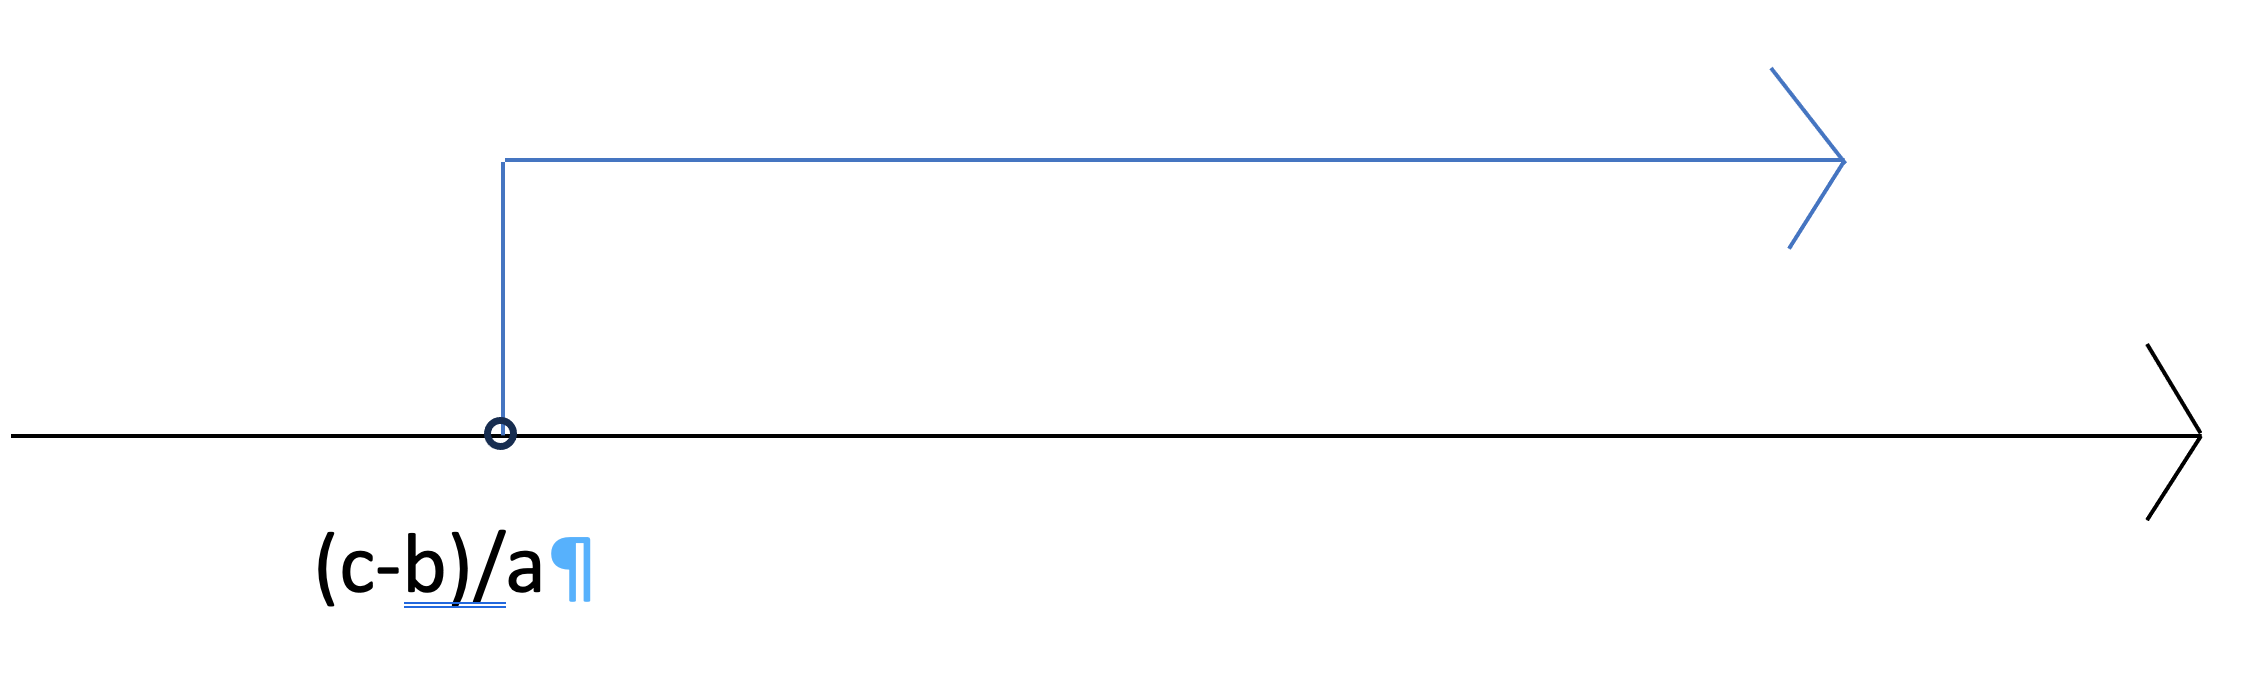
\includegraphics[width=3.125in,height=\textheight]{Desigualdad1.png}
\caption{Desigualdad \(ax+b>c\)}
\end{figure}

\begin{Ejem}
Supongamos se tiene la desigualdad $ax+b\leq c$, con $a\neq0$: 

\begin{eqnarray*}
ax+b&\leq&c\\
ax+b-b&\leq&c-b\\
ax&\leq&c-b\\
\left(\frac{1}{a}\right)ax&\leq&\left(\frac{1}{a}\right)\left(c-b\right)\\
\left(\frac{1}{a}\times a\right)x&\leq&\frac{c-b}{a}\\
\left(\frac{a}{a}\right)x&\leq&\frac{c-b}{a}\\
\left(1\right)x&\leq&\frac{c-b}{a}\\
x&\leq&\frac{c-b}{a}
\end{eqnarray*}
\begin{flushright}
$\blacksquare$
\end{flushright}

\end{Ejem}

\begin{figure}
\centering
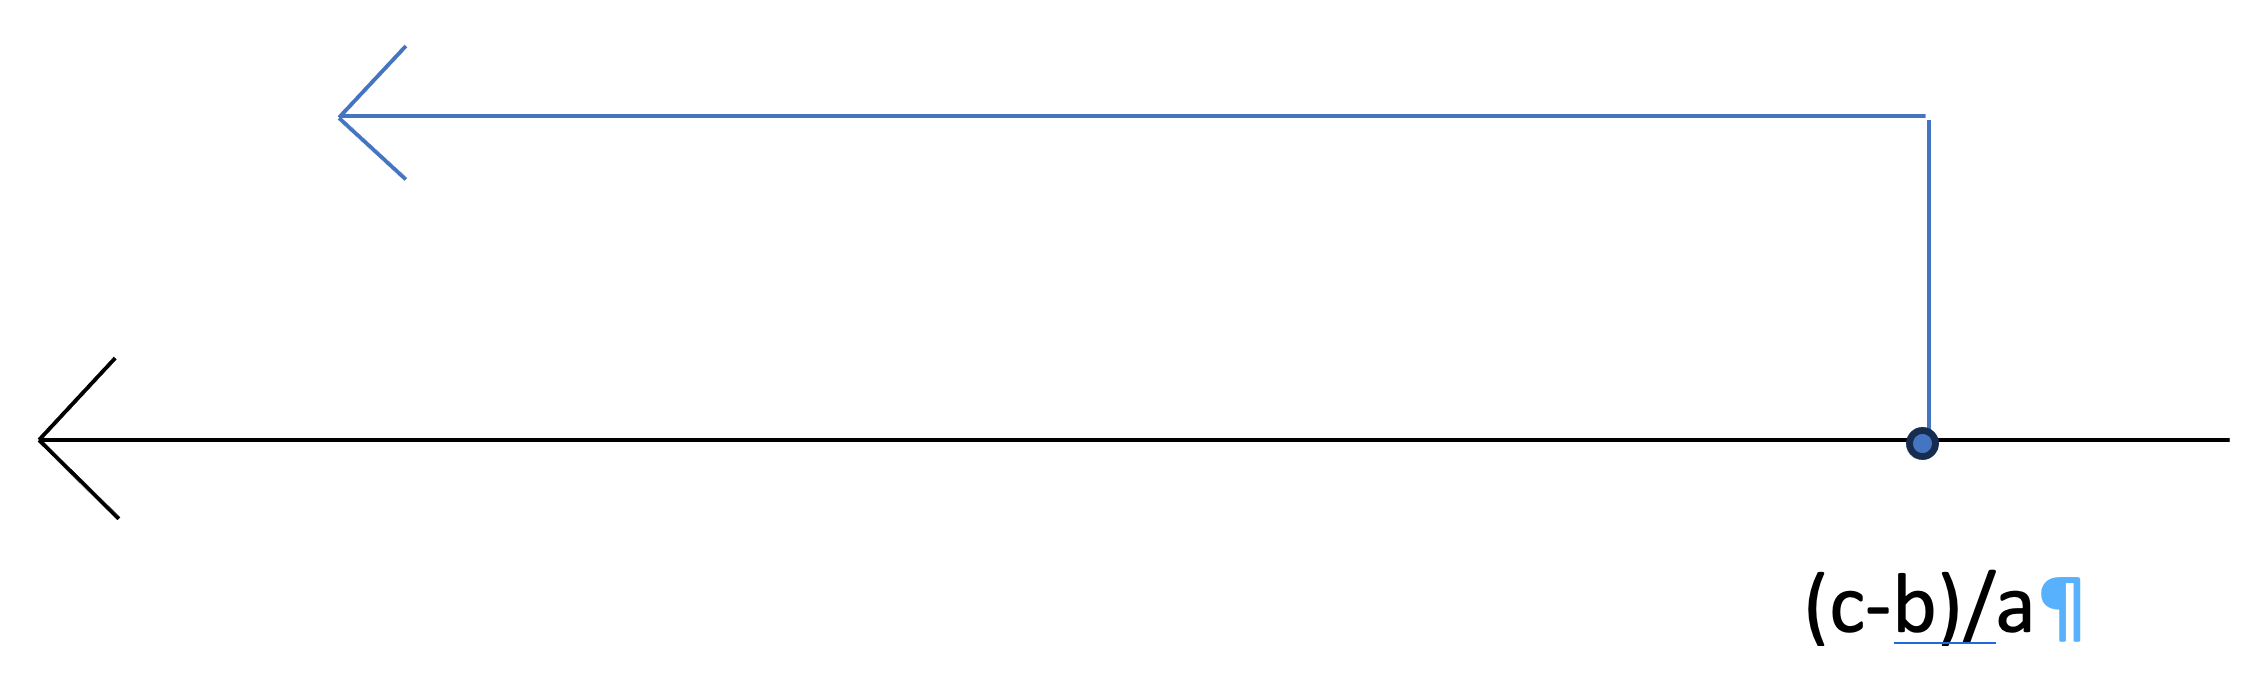
\includegraphics[width=3.125in,height=\textheight]{Desigualdad2.png}
\caption{Desigualdad \(ax+b\leq c\)}
\end{figure}

\begin{Ejem}
Supongamos se tiene la desigualdad $c\leq ax+b\leq d$, con $a\neq0$: 

\begin{eqnarray*}
c&\leq& ax+b<d\\
c-b&\leq& ax+b-b<d-b\\
c-b&\leq& ax+0<d-b\\
c-b&\leq& ax<d-b\\
\left(\frac{1}{a}\right)c-b&\leq& \left(\frac{1}{a}\right)ax<\left(\frac{1}{a}\right)d-b\\
\left(\frac{c-b}{a}\right)&\leq& \left(\frac{a}{a}\right)x<\left(\frac{d-b}{a}\right)\\
\left(\frac{c-b}{a}\right)&\leq& x<\left(\frac{d-b}{a}\right)\\
\end{eqnarray*}
\begin{flushright}
$\blacksquare$
\end{flushright}

\end{Ejem}

\begin{figure}
\centering
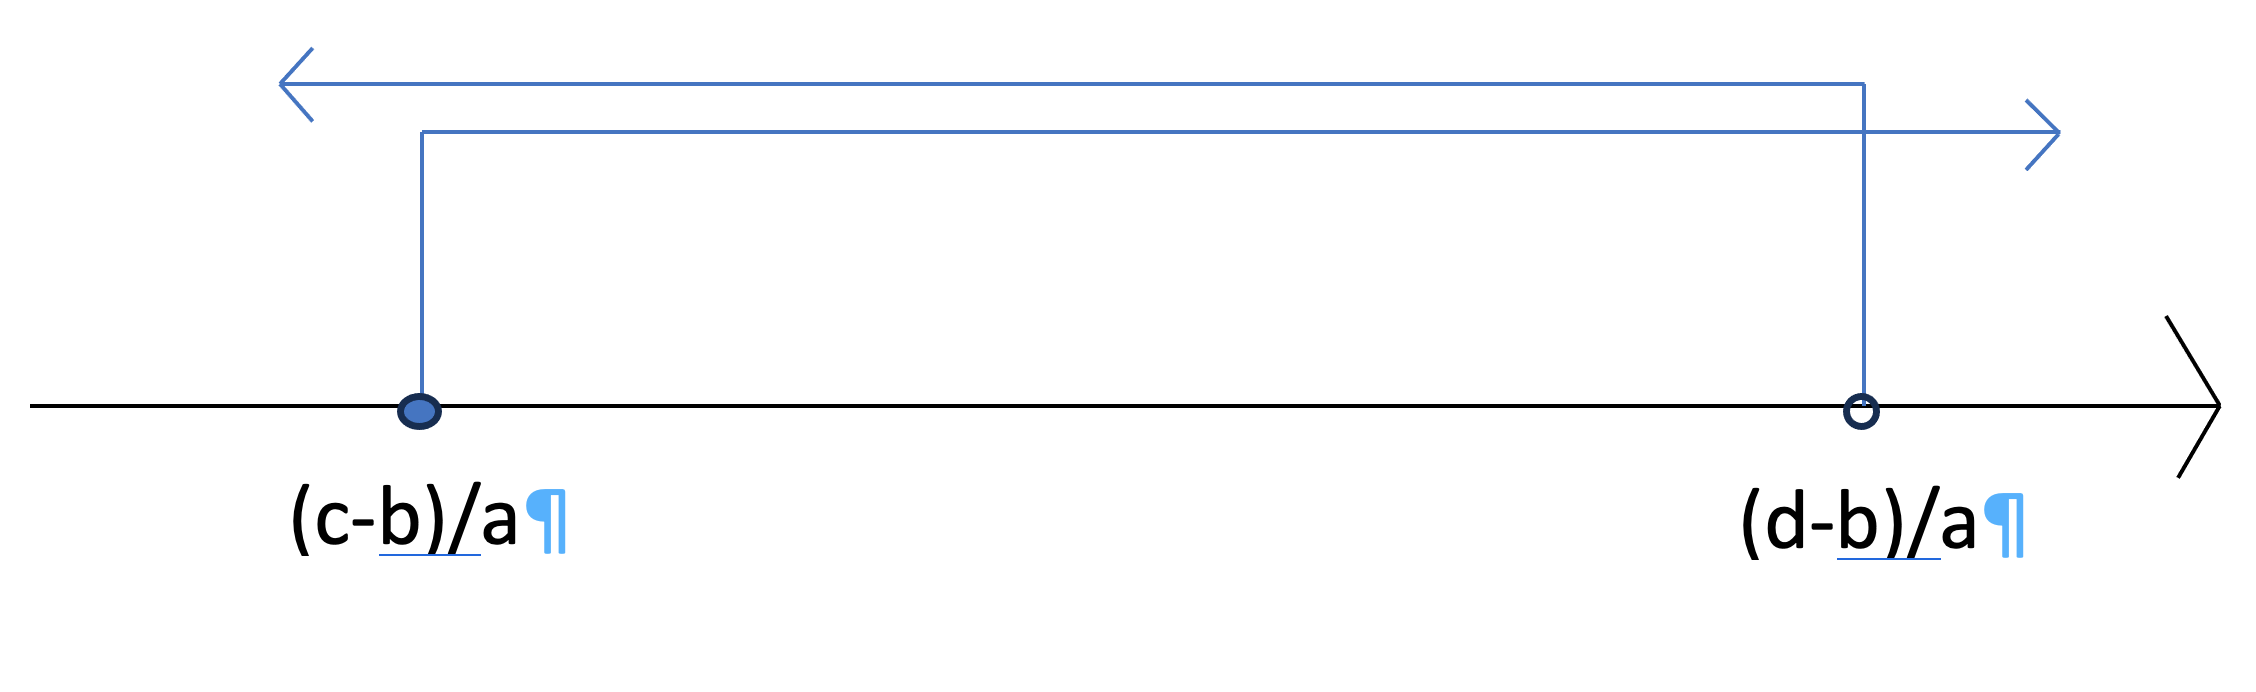
\includegraphics[width=3.125in,height=\textheight]{Desigualdad3.png}
\caption{Desigualdad \(c\leq ax+b\leq d\), con \(a\neq0\)}
\end{figure}

\begin{Ejem}
Supongamos se tiene la desigualdad $|ax+b|\leq c$, con $a\neq0$, recordemos que $|a|=b$, sí y sólo si $a=b$ o $a=-b$, entonces

\begin{eqnarray*}
|ax+b|&\leq& c\\
-c&\leq& ax+b \leq c\\
-c-b&\leq& ax+b-b \leq c-b\\
-c-b&\leq& ax+0<c-b\\
-c-b&\leq& ax<c-b\\
\left(\frac{1}{a}\right)c-b&\leq& \left(\frac{1}{a}\right)ax<\left(\frac{1}{a}\right)c-b\\
\left(\frac{-c-b}{a}\right)&\leq& \left(\frac{a}{a}\right)x<\left(\frac{c-b}{a}\right)\\
\left(\frac{-c-b}{a}\right)&\leq& x<\left(\frac{c-b}{a}\right)\\
-\left(\frac{c+b}{a}\right)&\leq& x<\left(\frac{c-b}{a}\right)\\
\end{eqnarray*}
\begin{flushright}
$\blacksquare$
\end{flushright}

\end{Ejem}

\begin{figure}
\centering
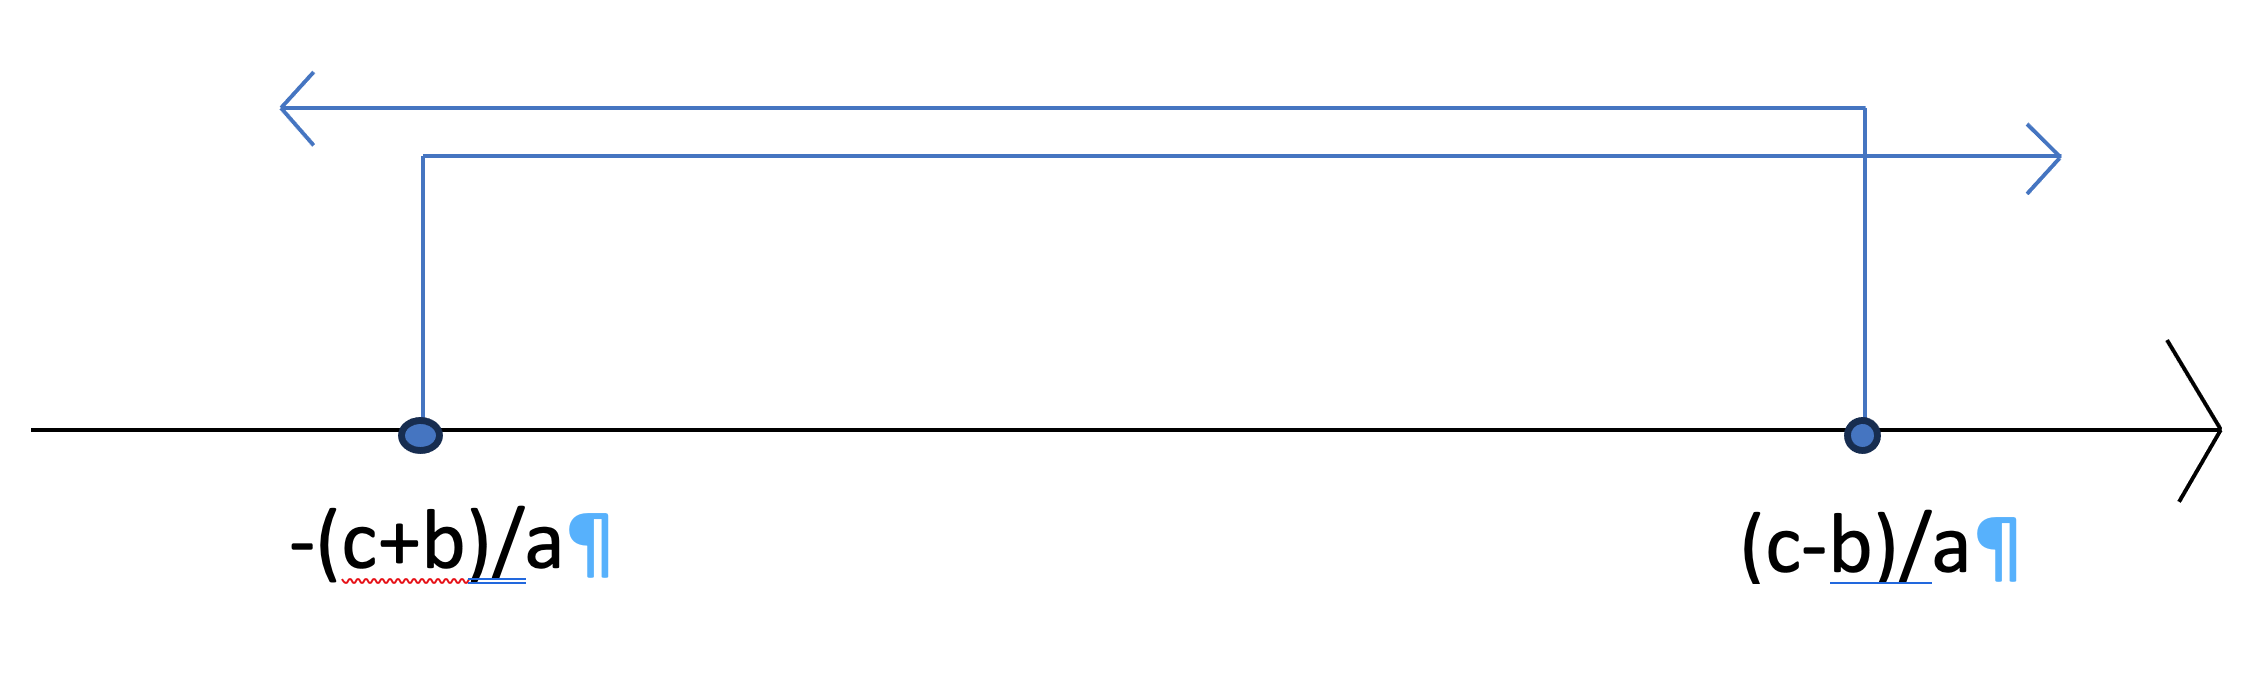
\includegraphics[width=3.125in,height=\textheight]{Desigualdad4.png}
\caption{Desigualdad \(|ax+b|\leq c\), con \(a\neq0\)}
\end{figure}

\begin{Ejem}
Supongamos se tiene la desigualdad $|ax+b|\geq c$, con $a\neq0$, recordemos que $|a|\geq b$ sí y sólo sí, $a\geq b$ o $a\leq -b$, entonces tenemos dos casos

\begin{itemize}
\item[Caso 1:]
\begin{eqnarray*}
ax+b&\geq& c\\
ax+b-b&\geq& c-b\\
ax+0&\geq& c-b\\
ax&\geq& c-b\\
\left(\frac{1}{a}\right)ax&\geq&\left(\frac{1}{a}\right)c-b\\
\left(\frac{a}{a}\right)ax&\geq&\left(\frac{1}{a}\right)c-b\\
\left(1\right)x&\geq&\left(\frac{c-b}{a}\right)\\
x&\geq&\left(\frac{c-b}{a}\right)
\end{eqnarray*}


\item[Caso 2:]
\begin{eqnarray*}
ax+b&\leq& -c\\
ax+b-b&\leq& -c-b\\
ax+0&\leq& -c-b\\
ax&\leq& -c-b\\
\left(\frac{1}{a}\right)ax&\leq&\left(\frac{1}{a}\right)\left(-c-b\right)\\
\left(\frac{a}{a}\right)ax&\leq&\left(\frac{1}{a}\right)\left(-c-b\right)\\
\left(1\right)x&\leq&-\left(\frac{c+b}{a}\right)\\
x&\leq&-\left(\frac{c+b}{a}\right)\\
\end{eqnarray*}

\end{itemize}

\begin{flushright}
$\blacksquare$
\end{flushright}

\end{Ejem}


\subsection{Solución de desigualdades de primer grado}

\subsubsection{Solución de desigualdades del tipo: \(ax+b>c\)}

\textbf{Resuelve las siguientes desigualdades, proporcionando el conjunto solución, el intervalo solución así como la representación gráfica de la misma}

\begin{enumerate}
\def\labelenumi{\arabic{enumi}.}
\item
  \(2x+3>7\)
\item
  \(-5x+2>9\)
\item
  \(4x-1>3\)
\item
  \(-3x+5>8\)
\item
  \(2x+1>3x-2\)
\item
  \(3x-2>2x+4\)
\item
  \(4x+1>2x+5\)
\item
  \(-2x-3>4x-7\)
\item
  \(5x-2>3x+4\)
\item
  \(2x+4>6x-8\)
\item
  \(-4x+3>5x-2\)
\item
  \(3x-1>4x-3\)
\item
  \(2x-5>x-3\)
\item
  \(3x+2>2x-5\)
\item
  \(-2x+1>5x-8\)
\end{enumerate}

\subsubsection{Solución de desigualdades del tipo: \(ax+b>c\), con coeficientes fraccionarios}

\textbf{Resuelve las siguientes desigualdades, proporcionando el conjunto solución, el intervalo solución así como la representación gráfica de la misma}

\begin{enumerate}
\def\labelenumi{\arabic{enumi}.}
\item
  \(\frac{1}{2}x+\frac{3}{4}>1\)
\item
  \(-\frac{2}{3}x+\frac{4}{5}>3\)
\item
  \(\frac{3}{4}x-\frac{1}{2}>\frac{5}{6}\)
\item
  \(-\frac{2}{5}x+\frac{1}{3}>-\frac{1}{15}\)
\item
  \(\frac{2}{3}x+\frac{1}{4}>\frac{5}{6}x-\frac{1}{2}\)
\item
  \(\frac{1}{2}x-\frac{1}{3}>-\frac{2}{5}x+\frac{7}{15}\)
\item
  \(-\frac{3}{4}x+\frac{1}{2}>\frac{2}{3}x-\frac{1}{4}\)
\item
  \(\frac{1}{3}x-\frac{2}{5}>\frac{2}{7}x-\frac{1}{7}\)
\item
  \(\frac{2}{5}x+\frac{1}{6}\geq\frac{1}{3}x+\frac{5}{6}\)
\item
  \(\frac{3}{4}x+\frac{1}{5}>\frac{1}{2}x+\frac{3}{10}\)
\item
  \(-\frac{1}{2}x+\frac{1}{3}>-\frac{3}{4}x-\frac{1}{6}\)
\item
  \(\frac{1}{4}x-\frac{1}{2}>\frac{2}{3}x-\frac{4}{6}\)
\item
  \(\frac{2}{3}x-\frac{1}{4}>\frac{3}{4}x-\frac{2}{3}\)
\item
  \(-\frac{1}{2}x+\frac{3}{4}>\frac{3}{5}x+\frac{1}{10}\)
\item
  \(\frac{2}{5}x-\frac{1}{4}>-\frac{1}{2}x+\frac{3}{8}\)
\end{enumerate}

\subsubsection{\texorpdfstring{Solución de desigualdades del tipo:
\(ax+b<c\)}{Solución de desigualdades del tipo: ax+b\textless c}}\label{soluciuxf3n-de-desigualdades-del-tipo-axbc-1}

\textbf{Resuelve las siguientes desigualdades, proporcionando el
conjunto solución, el intervalo solución así como la representación
gráfica de la misma}

\begin{enumerate}
\def\labelenumi{\arabic{enumi}.}
\item
  \(2x+3<7\)
\item
  \(-5x+2<-9\)
\item
  \(4x-1<3\)
\item
  \(-3x+5<8\)
\item
  \(2x+1<3x-2\)
\item
  \(3x-2<2x+4\)
\item
  \(4x+1<2x+5\)
\item
  \(-2x-3<4x-7\)
\item
  \(5x-2<3x+4\)
\item
  \(2x+4<6x-8\)
\item
  \(-4x+3<5x-2\)
\item
  \(3x-1<4x-3\)
\item
  \(2x-5<x-3\)
\item
  \(3x+2<2x-5\)
\item
  \(-2x+1<5x-8\)
\end{enumerate}

\subsubsection{Solución de desigualdades del tipo: \(ax+b<c\) con coeficientes fraccionarios}
\textbf{Resuelve las siguientes desigualdades, proporcionando el conjunto solución, el intervalo solución así como la representación gráfica de la misma}

\begin{enumerate}
\def\labelenumi{\arabic{enumi}.}
\item
  \(\frac{1}{2}x+\frac{3}{4}<\frac{5}{8}\)
\item
  \(-\frac{2}{3}x+\frac{4}{5}<\frac{1}{2}\)
\item
  \(\frac{3}{4}x-\frac{1}{2}<\frac{5}{6}\)
\item
  \(-\frac{2}{5}x+\frac{1}{3}<-\frac{1}{15}\)
\item
  \(\frac{2}{3}x+\frac{1}{4}<\frac{5}{6}x-\frac{1}{2}\)
\item
  \(\frac{1}{2}x-\frac{1}{3}<\frac{2}{5}x-\frac{7}{15}\)
\item
  \(-\frac{3}{4}x+\frac{1}{2}<\frac{2}{3}x-\frac{1}{4}\)
\item
  \(\frac{1}{3}x-\frac{2}{5}<\frac{2}{7}x-\frac{1}{7}\)
\item
  \(\frac{2}{5}x+\frac{1}{6}<\frac{1}{3}x+\frac{5}{6}\)
\item
  \(\frac{3}{4}x+\frac{1}{5}<\frac{1}{2}x+\frac{3}{10}\)
\item
  \(-\frac{1}{2}x+\frac{1}{3}<-\frac{3}{4}x-\frac{1}{6}\)
\item
  \(\frac{1}{4}x-\frac{1}{2}<\frac{2}{3}x-\frac{4}{6}\)
\item
  \(\frac{2}{3}x-\frac{1}{4}<\frac{3}{4}x-\frac{2}{3}\)
\item
  \(-\frac{1}{2}x+\frac{3}{4}<\frac{3}{5}x+\frac{1}{10}\)
\item
  \(\frac{2}{5}x-\frac{1}{4}<-\frac{1}{2}x+\frac{3}{8}\)
\end{enumerate}

\subsubsection{Solución de desigualdades del tipo: \(ax+b \geq c\)}

\textbf{Resuelve las siguientes desigualdades, proporcionando el conjunto solución, el intervalo solución así como la representación gráfica de la misma}

\begin{enumerate}
\def\labelenumi{\arabic{enumi}.}
\item
  \(2x + 3 \geq 5\)
\item
  \(-4x + 2 \geq -10\)
\item
  \(5x - 4 \geq 6\)
\item
  \(-3x + 7 \geq 4\)
\item
  \(2x - 3 \geq x + 2\)
\item
  \(3x + 2 \geq 2x - 1\)
\item
  \(4x - 1 \geq x + 5\)
\item
  \(-2x - 3 \geq -6x - 1\)
\item
  \(5x - 2 \geq 2x + 8\)
\item
  \(2x + 4 \geq 4x - 2\)
\item
  \(-4x + 3 \geq 3x - 2\)
\item
  \(3x - 1 \geq 2x + 1\)
\item
  \(2x - 5 \geq x - 1\)
\item
  \(3x + 2 \geq 2x - 4\)
\item
  \(-2x + 1 \geq -5x + 4\)
\end{enumerate}

\subsubsection{Solución de desigualdades del tipo: \(ax+b \geq c\), con coeficientes fraccionarios}{
\textbf{Resuelve las siguientes desigualdades, proporcionando el conjunto solución, el intervalo solución así como la representación gráfica de la misma}

\begin{enumerate}
\def\labelenumi{\arabic{enumi}.}
\item
  \(\frac{1}{2}x + \frac{3}{4} \geq \frac{5}{8}\)
\item
  \(-\frac{2}{3}x + \frac{4}{5} \geq \frac{1}{2}\)
\item
  \(\frac{3}{4}x - \frac{1}{2} \geq \frac{5}{6}\)
\item
  \(-\frac{2}{5}x + \frac{1}{3} \geq -\frac{1}{15}\)
\item
  \(\frac{2}{3}x + \frac{1}{4} \geq \frac{5}{6}x - \frac{1}{2}\)
\item
  \(\frac{1}{2}x - \frac{1}{3} \geq \frac{2}{5}x - \frac{7}{15}\)
\item
  \(-\frac{3}{4}x + \frac{1}{2} \geq \frac{2}{3}x - \frac{1}{4}\)
\item
  \(\frac{1}{3}x - \frac{2}{5} \geq \frac{2}{7}x - \frac{1}{7}\)
\item
  \(\frac{2}{5}x + \frac{1}{6} \geq \frac{1}{3}x + \frac{5}{6}\)
\item
  \(\frac{3}{4}x + \frac{1}{5} \geq \frac{1}{2}x + \frac{3}{10}\)
\item
  \(-\frac{1}{2}x + \frac{1}{3} \geq -\frac{3}{4}x - \frac{1}{6}\)
\item
  \(\frac{1}{4}x - \frac{1}{2} \geq \frac{2}{3}x - \frac{4}{6}\)
\item
  \(\frac{2}{3}x - \frac{1}{4} \geq \frac{3}{4}x - \frac{2}{3}\)
\item
  \(-\frac{1}{2}x + \frac{3}{4} \geq \frac{3}{5}x + \frac{1}{10}\)
\item
  \(\frac{2}{5}x - \frac{1}{4} \geq -\frac{1}{2}x + \frac{3}{8}\)
\end{enumerate}

\subsubsection{Solución de desigualdades del tipo: \(ax+b \leq c\)}

\textbf{Resuelve las siguientes desigualdades, proporcionando el conjunto solución, el intervalo solución así como la representación gráfica de la misma}

\begin{enumerate}
\def\labelenumi{\arabic{enumi}.}
\item
  \(2x + 3 \leq 7\)
\item
  \(-3x + 4 \leq 5\)
\item
  \(4x - 2 \leq 6\)
\item
  \(-5x + 3 \leq 2\)
\item
  \(2x + 1 \leq 5x - 2\)
\item
  \(3x - 1 \leq 5x + 2\)
\item
  \(-4x + 2 \leq 3x + 1\)
\item
  \(3x - 5 \leq 7x - 2\)
\item
  \(5x + 1 \leq 3x + 4\)
\item
  \(4x + 1 \leq 6x - 3\)
\item
  \(-2x + 3 \leq -4x - 1\)
\item
  \(x - 2 \leq 2x + 1\)
\item
  \(3x - 4 \leq 4x - 2\)
\item
  \(-2x + 4 \leq 5x + 1\)
\item
  \(2x - 1 \leq -3x + 4\)
\end{enumerate}

\subsubsection{Solución de desigualdades del tipo: \(ax+b \leq c\) con coeficientes fraccionarios.}
\textbf{Resuelve las siguientes desigualdades, proporcionando el conjunto solución, el intervalo solución así como la representación gráfica de la misma}

\begin{enumerate}
\def\labelenumi{\arabic{enumi}.}
\item
  \(\frac{1}{2}x + \frac{3}{4} \leq \frac{5}{8}\)
\item
  \(-\frac{2}{3}x + \frac{4}{5} \leq \frac{1}{2}\)
\item
  \(\frac{3}{4}x - \frac{1}{2} \leq \frac{5}{6}\)
\item
  \(-\frac{2}{5}x + \frac{1}{3} \leq -\frac{1}{15}\)
\item
  \(\frac{2}{3}x + \frac{1}{4} \leq \frac{5}{6}x - \frac{1}{2}\)
\item
  \(\frac{1}{2}x - \frac{1}{3} \leq \frac{2}{5}x - \frac{7}{15}\)
\item
  \(-\frac{3}{4}x + \frac{1}{2} \leq \frac{2}{3}x - \frac{1}{4}\)
\item
  \(\frac{1}{3}x - \frac{2}{5} \leq \frac{2}{7}x - \frac{1}{7}\)
\item
  \(\frac{2}{5}x + \frac{1}{6} \leq \frac{1}{3}x + \frac{5}{6}\)
\item
  \(\frac{3}{4}x + \frac{1}{5} \leq \frac{1}{2}x + \frac{3}{10}\)
\item
  \(-\frac{1}{2}x + \frac{1}{3} \leq -\frac{3}{4}x - \frac{1}{6}\)
\item
  \(\frac{1}{4}x - \frac{1}{2} \leq \frac{2}{3}x - \frac{4}{6}\)
\item
  \(\frac{2}{3}x - \frac{1}{4} \leq \frac{3}{4}x - \frac{2}{3}\)
\item
  \(-\frac{1}{2}x + \frac{3}{4} \leq \frac{3}{5}x + \frac{1}{10}\)
\item
  \(\frac{2}{5}x - \frac{1}{4} \leq -\frac{1}{2}x + \frac{3}{8}\)
\end{enumerate}

\subsection{Solución de desigualdades con doble desigualdad.} 

\subsubsection{Solución de desigualdades del tipo: \(c< ax+b <d\)}
\textbf{Resuelve las siguientes desigualdades, proporcionando el conjunto solución, el intervalo solución así como la representación gráfica de la misma}

\begin{enumerate}
\def\labelenumi{\arabic{enumi}.}
\item
  \(2<x+3<5\)
\item
  \(-1<2x-1<1\)
\item
  \(-\frac{1}{2}<\frac{3}{4}x+\frac{1}{2}<\frac{1}{2}\)
\item
  \(-3< 2x+7<-1\)
\item
  \(1<\frac{1}{2}x-\frac{1}{4}<2\)
\item
  \(-5<-\frac{1}{3}x+\frac{5}{6}<1\)
\item
  \(-5<5x-1<8\)
\item
  \(-2< \frac{2}{3}x+1<12\)
\item
  \(2<-\frac{1}{2}x+\frac{3}{4}<3\)
\item
  \(-3< \frac{1}{2}x-\frac{1}{3}<18\)
\item
  \(-4< -3x+5<3\)
\item
  \(1<\frac{1}{2}x+\frac{1}{3}<2\)
\item
  \(-2< 4x-1<2\)
\item
  \(-\frac{3}{4}<\frac{1}{2}x-\frac{1}{4}<\frac{3}{4}\)
\item
  \(-1<s\frac{3}{2}x+1<2\)
\end{enumerate}

\subsubsection{Solución de desigualdades del tipo: \(c< ax+b \leq d\)}

\textbf{Resuelve las siguientes desigualdades, proporcionando el conjunto solución, el intervalo solución así como la representación gráfica de la misma}

\begin{enumerate}
\def\labelenumi{\arabic{enumi}.}
\item
  \(-2<3x+1\leq 5\)
\item
  \(-\frac{4}{5}< \frac{1}{2}x-\frac{3}{4}\leq2\)
\item
  \(-1<2x-1\leq 1\)
\item
  \(-3< \frac{1}{2}x+\frac{1}{3}\leq \frac{8}{5}\)
\item
  \(-\frac{3}{4}<\frac{1}{2}x+\frac{1}{4}\leq \frac{3}{4}\)
\item
  \(-2<\frac{3}{2}x-1\leq 1\)
\item
  \(-1<\frac{2}{3}x+1\leq \frac{8}{3}\)
\item
  \(1<\frac{1}{2}x+\frac{1}{3}\leq 2\)
\item
  \(-3< -2x+5\leq 3\)
\item
  \(-\frac{1}{2}<\frac{3}{4}x+\frac{1}{2}\leq \frac{1}{2}\)
\item
  \(-5<5x-1\leq 9\)
\item
  \(1<\frac{1}{2}x-\frac{1}{4}\leq 2\)
\item
  \(-3< 2x+7\leq -1\)
\item
  \(-1< -\frac{1}{2}x+\frac{1}{4}\leq 2\)
\item
  \(2<-\frac{1}{2}x+\frac{3}{4}\leq 3\)
\end{enumerate}

\subsubsection{Solución de desigualdades del tipo: \(c\leq ax+b <d\)}

\textbf{Resuelve las siguientes desigualdades, proporcionando el conjunto solución, el intervalo solución así como la representación gráfica de la misma}

\begin{enumerate}
\def\labelenumi{\arabic{enumi}.}
\item
  \(-2\leq 3x+1<5\)
\item
  \(-\frac{4}{5}\leq \frac{1}{2}x-\frac{3}{4}<2\)
\item
  \(-1\leq 2x-1<1\)
\item
  \(-3\leq \frac{1}{2}x+\frac{1}{3}<\frac{7}{9}\)
\item
  \(-\frac{3}{4}\leq \frac{1}{2}x+\frac{1}{4}<\frac{3}{4}\)
\item
  \(-2\leq \frac{3}{2}x-1<1\)
\item
  \(-1\leq \frac{2}{3}x+1<\frac{9}{4}\)
\item
  \(1\leq \frac{1}{2}x+\frac{1}{3}<2\)
\item
  \(-\frac{4}{3}\leq -2x+5<3\)
\item
  \(-\frac{1}{2}\leq \frac{3}{4}x+\frac{1}{2}<\frac{1}{2}\)
\item
  \(-5\leq 5x-1<\frac{15}{6}\)
\item
  \(1\leq \frac{1}{2}x-\frac{1}{4}<2\)
\item
  \(-3\leq 2x+7<-1\)
\item
  \(-1\leq -\frac{1}{2}x+\frac{1}{4}<2\)
\item
  \(2\leq -\frac{1}{2}x+\frac{3}{4}<3\)
\end{enumerate}

\subsubsection{Solución de desigualdades del tipo: \(c\leq ax+b \leq d\)}
\textbf{Resuelve las siguientes desigualdades, proporcionando el conjunto solución, el intervalo solución así como la representación gráfica de la misma}

\begin{enumerate}
\def\labelenumi{\arabic{enumi}.}
\item
  \(-1\leq x\leq 2\)
\item
  \(-\frac{3}{4}\leq \frac{1}{2}x+\frac{1}{4}\leq \frac{5}{8}\)
\item
  \(2\leq 3x-1\leq 7\)
\item
  \(-\frac{1}{3}\leq \frac{1}{6}x+\frac{1}{2}\leq \frac{1}{2}\)
\item
  \(-1\leq -x+3\leq 2\)
\item
  \(-2\leq \frac{1}{2}x+1\leq 3\)
\item
  \(2\leq \frac{3}{2}x+1\leq 5\)
\item
  \(-\frac{3}{4}\leq -\frac{1}{2}x+\frac{1}{4}\leq \frac{1}{4}\)
\item
  \(-4\leq 2x+1\leq 7\)
\item
  \(-\frac{1}{2}\leq -\frac{3}{4}x+\frac{1}{2}\leq 1\)
\item
  \(-\frac{5}{2}\leq \frac{1}{4}x+1\leq 1\)
\item
  \(1\leq -\frac{1}{2}x+\frac{3}{4}\leq 3\)
\item
  \(-\frac{5}{6}\leq \frac{1}{3}x+\frac{1}{2}\leq \frac{1}{2}\)
\item
  \(-1\leq \frac{1}{2}x-\frac{1}{4}\leq 3\)
\item
  \(-2\leq \frac{1}{4}x+\frac{1}{2}\leq 3\)
\end{enumerate}

\subsection{Solución de desigualdades con valor absoluto}

\subsubsection{Solución de desigualdades del tipo: \(|ax+b| <d\)}

\textbf{Resuelve las siguientes desigualdades, proporcionando el conjunto solución, el intervalo solución así como la representación gráfica de la misma}

\begin{enumerate}
\def\labelenumi{\arabic{enumi}.}
\item
  \(|2x+1|<5\)
\item
  \(|\frac{1}{2}x-\frac{1}{4}|<2\)
\item
  \(|3x-1|<7\)
\item
  \(|\frac{1}{3}x+\frac{1}{2}|<1\)
\item
  \(|x-2|<4\)
\item
  \(|\frac{1}{2}x+1|<3\)
\item
  \(|\frac{3}{2}x+1|<5\)
\item
  \(|\frac{1}{2}x-\frac{1}{4}|<\frac{3}{4}\)
\item
  \(|2x+1|<6\)
\item
  \(|\frac{3}{4}x-\frac{1}{2}|<1\)
\item
  \(|\frac{1}{4}x+1|<\frac{7}{2}\)
\item
  \(|-\frac{1}{2}x+\frac{3}{4}|<2\)
\item
  \(|\frac{1}{3}x+\frac{1}{2}|<\frac{5}{6}\)
\item
  \(|\frac{1}{2}x-\frac{1}{4}|<3\)
\item
  \(|\frac{1}{4}x+\frac{1}{2}|<\frac{7}{4}\)
\end{enumerate}

\subsubsection{Solución de desigualdades del tipo: \(|ax+b| \leq d\)}
\textbf{Resuelve las siguientes desigualdades, proporcionando el conjunto solución, el intervalo solución así como la representación gráfica de la misma}

\begin{enumerate}
\def\labelenumi{\arabic{enumi}.}
\item
  \(|3x-1|\leq 6\)
\item
  \(|\frac{1}{2}x-\frac{1}{4}|\leq 1\)
\item
  \(|2x+1|\leq 5\)
\item
  \(|\frac{1}{3}x+\frac{1}{2}|\leq \frac{4}{3}\)
\item
  \(|x-2|\leq 3\)
\item
  \(|\frac{1}{2}x+1|\leq 4\)
\item
  \(|\frac{3}{2}x+1|\leq 5\)
\item
  \(|\frac{1}{2}x-\frac{1}{4}|\leq \frac{5}{4}\)
\item
  \(|2x+1|\leq 7\)
\item
  \(|\frac{3}{4}x-\frac{1}{2}|\leq 2\)
\item
  \(|\frac{1}{4}x+1|\leq 3\)
\item
  \(|-\frac{1}{2}x+\frac{3}{4}|\leq 2\)
\item
  \(|\frac{1}{3}x+\frac{1}{2}|\leq 1\)
\end{enumerate}


\subsubsection{Solución de desigualdades del tipo: \(|ax+b| >d\)}
\textbf{Resuelve las siguientes desigualdades, proporcionando el conjunto solución, el intervalo solución así como la representación gráfica de la misma}

\begin{enumerate}
\def\labelenumi{\arabic{enumi}.}
\item
  \(|3x-1|>4\)
\item
  \(|\frac{1}{2}x-\frac{1}{4}|>\frac{1}{2}\)
\item
  \(|2x+1|>3\)
\item
  \(|\frac{1}{3}x+\frac{1}{2}|>\frac{5}{6}\)
\item
  \(|x-2|>1\)
\item
  \(|\frac{1}{2}x+1|>\frac{3}{4}\)
\item
  \(|\frac{3}{2}x+1|>\frac{7}{2}\)
\item
  \(|\frac{1}{2}x-\frac{1}{4}|>\frac{3}{4}\)
\item
  \(|2x+1|>\frac{9}{2}\)
\item
  \(|\frac{3}{4}x-\frac{1}{2}|>\frac{5}{4}\)
\item
  \(|\frac{1}{4}x+1|>1\)
\item
  \(|-\frac{1}{2}x+\frac{3}{4}|>\frac{1}{2}\)
\item
  \(|\frac{1}{3}x+\frac{1}{2}|>\frac{2}{3}\)
\item
  \(|\frac{1}{2}x-\frac{1}{4}|>\frac{5}{4}\)
\item
  \(|\frac{1}{4}x+\frac{1}{2}|>1\)
\end{enumerate}

\subsubsection{Solución de desigualdades del tipo: \(|ax+b| \geq d\)}

\textbf{Resuelve las siguientes desigualdades, proporcionando el conjunto solución, el intervalo solución así como la representación gráfica de la misma}

\begin{enumerate}
\def\labelenumi{\arabic{enumi}.}
\item
  \(|3x-1|\geq 4\)
\item
  \(|\frac{1}{2}x-\frac{1}{4}|\geq\frac{1}{2}\)
\item
  \(|2x+1|\geq 3\)
\item
  \(|\frac{1}{3}x+\frac{1}{2}|\geq\frac{5}{6}\)
\item
  \(|x-2|\geq 1\)
\item
  \(|\frac{1}{2}x+1|\geq\frac{3}{4}\)
\item
  \(|\frac{3}{2}x+1|\geq\frac{7}{2}\)
\item
  \(|\frac{1}{2}x-\frac{1}{4}|\geq\frac{3}{4}\)
\item
  \(|2x+1|\geq\frac{9}{2}\)
\item
  \(|\frac{3}{4}x-\frac{1}{2}|\geq\frac{5}{4}\)
\item
  \(|\frac{1}{4}x+1|\geq 1\)
\item
  \(|-\frac{1}{2}x+\frac{3}{4}|\geq\frac{1}{2}\)
\item
  \(|\frac{1}{3}x+\frac{1}{2}|\geq\frac{2}{3}\)
\item
  \(|\frac{1}{2}x-\frac{1}{4}|\geq\frac{5}{4}\)
\item
  \(|\frac{1}{4}x+\frac{1}{2}|\geq 1\)
\end{enumerate}

\subsection{Ejercicios adicionales}

\begin{enumerate}
\def\labelenumi{\arabic{enumi}.}
\item
  Resuelve los ejercicios siguientes, encuentra el intervalo solución y
  proporciona su gráfica

  \begin{enumerate}
  \def\labelenumii{\roman{enumii}.}
  \tightlist
  \item
    \(|-\frac{1}{3}x+\frac{2}{5}| \leq \frac{4}{5}\)
  \item
    \(|-\frac{2}{7}x-\frac{3}{4}| \leq \frac{2}{3}\)
  \item
    \(|\frac{5}{8}x-\frac{1}{6}| \leq \frac{7}{8}\)
  \item
    \(|\frac{3}{10}x+\frac{2}{9}| \leq \frac{1}{2}\)
  \item
    \(|-\frac{4}{11}x+\frac{5}{7}| \leq \frac{3}{4}\)
  \item
    \(|-\frac{2}{5}x-\frac{1}{3}| \leq \frac{2}{5}\)
  \item
    \(|\frac{1}{6}x+\frac{7}{9}| \leq \frac{1}{3}\)
  \item
    \(|\frac{7}{9}x-\frac{4}{11}| \leq \frac{5}{6}\)
  \item
    \(|-\frac{5}{8}x+\frac{3}{10}| \leq \frac{2}{7}\)
  \item
    \(|-\frac{1}{4}x-\frac{1}{8}| \leq \frac{3}{4}\)
  \item
    \(|\frac{3}{7}x+\frac{5}{6}| \leq \frac{1}{5}\)
  \item
    \(|-\frac{4}{9}x+\frac{2}{11}| \leq \frac{4}{9}\)
  \item
    \(|-\frac{2}{5}x-\frac{7}{8}| \leq \frac{2}{3}\)
  \item
    \(|\frac{5}{11}x+\frac{1}{7}| \leq \frac{5}{11}\)
  \item
    \(|\frac{3}{8}x-\frac{2}{9}| \leq \frac{3}{4}\)
  \end{enumerate}
\item
  Realiza lo mismo para los siguientes ejercicios

  \begin{enumerate}
  \def\labelenumii{\roman{enumii}.}
  \tightlist
  \item
    \(|-\frac{2}{5}x+\frac{3}{4}| \leq \frac{1}{2}\)
  \item
    \(|\frac{3}{7}x+\frac{1}{8}| \leq \frac{2}{7}\)
  \item
    \(|-{\frac{5}{6}x-\frac{4}{9}}| \leq \frac{5}{6}\)
  \item
    \(|-\frac{4}{9}x+\frac{2}{11}| \leq \frac{3}{4}\)
  \item
    \(|-\frac{1}{3}x-\frac{2}{7}| \leq \frac{3}{5}\)
  \item
    \(|\frac{3}{8}x-\frac{1}{6}| \leq \frac{2}{5}\)
  \item
    \(|-{\frac{2}{7}x+\frac{5}{8}}| \leq \frac{3}{7}\)
  \item
    \(|\frac{5}{11}x+\frac{1}{3}| \leq \frac{4}{11}\)
  \item
    \(|-\frac{4}{5}x-\frac{3}{10}| \leq \frac{1}{4}\)
  \item
    \(|-\frac{1}{4}x+\frac{7}{9}| \leq \frac{5}{8}\)
  \item
    \(|-{\frac{2}{9}x-\frac{1}{5}}| \leq \frac{2}{9}\)
  \item
    \(|-\frac{3}{10}x+\frac{2}{7}| \leq \frac{4}{9}\)
  \item
    \(|\frac{5}{8}x-\frac{1}{3}| \leq \frac{3}{8}\)
  \item
    \(|\frac{4}{11}x+\frac{5}{6}| \leq \frac{2}{5}\)
  \item
    \(|-\frac{2}{5}x-\frac{3}{8}| \leq \frac{5}{6}\)
  \item
    \(|\frac{1}{6}x-\frac{2}{9}| \leq \frac{1}{4}\)
  \item
    \(|-{\frac{5}{9}x+\frac{4}{11}}| \leq \frac{2}{3}\)
  \item
    \(|-\frac{3}{8}x+\frac{1}{5}| \leq \frac{3}{8}\)
  \item
    \(|-\frac{4}{7}x-\frac{3}{10}| \leq \frac{1}{7}\)
  \item
    \(|-\frac{2}{11}x+\frac{5}{8}| \leq \frac{3}{10}\)
  \end{enumerate}
\item
  Finalmente realiza lo mismo para la siguiente lista:

  \begin{enumerate}
  \def\labelenumii{\roman{enumii}.}
  \tightlist
  \item
    \(|{-\frac{4}{9}x+\frac{5}{8}}| \geq \frac{1}{3}\)
  \item
    \(|{-\frac{1}{6}x-\frac{2}{7}}| > \frac{2}{5}\)
  \item
    \(|{\frac{7}{11}x+\frac{1}{8}}| \leq \frac{3}{7}\)
  \item
    \(|{-\frac{3}{8}x+\frac{4}{9}}| < \frac{5}{8}\)
  \item
    \(|{-\frac{5}{6}x+\frac{3}{10}}| \geq \frac{2}{3}\)
  \item
    \(|{-\frac{2}{7}x-\frac{1}{4}}| \leq \frac{5}{6}\)
  \item
    \(|{-\frac{1}{3}x+\frac{5}{9}}| > \frac{2}{7}\)
  \item
    \(|{\frac{4}{11}x-\frac{3}{8}}| \leq \frac{1}{5}\)
  \item
    \(|{-\frac{2}{9}x+\frac{1}{7}}| \geq \frac{3}{4}\)
  \item
    \(|{-\frac{5}{8}x+\frac{2}{11}}| < \frac{4}{9}\)
  \item
    \(|{\frac{1}{4}x+\frac{7}{9}}| \leq \frac{2}{7}\)
  \item
    \(|{-\frac{3}{10}x-\frac{5}{6}}| > \frac{1}{3}\)
  \item
    \(|{-\frac{4}{5}x+\frac{1}{6}}| \geq \frac{2}{5}\)
  \item
    \(|{-\frac{3}{7}x+\frac{4}{9}}| < \frac{3}{7}\)
  \item
    \(|{\frac{5}{11}x-\frac{2}{8}}| \leq \frac{4}{11}\)
  \item
    \(|{-\frac{2}{11}x-\frac{3}{8}}| > \frac{1}{6}\)
  \item
    \(|{-\frac{5}{9}x+\frac{2}{7}}| \geq \frac{3}{4}\)
  \item
    \(|{-\frac{3}{8}x-\frac{1}{6}}| < \frac{5}{11}\)
  \item
    \(|{\frac{4}{7}x+\frac{1}{5}}| \leq \frac{3}{10}\)
  \item
    \(|{-\frac{1}{5}x+\frac{6}{11}}| > \frac{2}{9}\)
  \end{enumerate}
\item
  Un poco más de ejercicios finales

  \begin{enumerate}
  \def\labelenumii{\roman{enumii}.}
  \tightlist
  \item
    \(|\frac{3x+2}{5}| \geq \frac{1}{4}\)
  \item
    \(|-\frac{6x-1}{2}| \leq \frac{3}{5}\)
  \item
    \(|\frac{-2x+9}{7}| > \frac{4}{9}\)
  \item
    \(|-\frac{-5x-3}{4}| \geq \frac{2}{7}\)
  \item
    \(|\frac{4x+7}{3}| < \frac{5}{6}\)
  \item
    \(|-\frac{9x-2}{8}| \leq \frac{7}{10}\)
  \item
    \(|\frac{-8x+3}{6}| > \frac{1}{5}\)
  \item
    \(|\frac{-7x-5}{9}| \geq \frac{2}{11}\)
  \item
    \(|-\frac{12x+4}{11}| < \frac{3}{8}\)
  \item
    \(|\frac{11x-6}{10}| \leq \frac{5}{9}\)
  \item
    \(|\frac{-15x+2}{13}| > \frac{4}{11}\)
  \item
    \(|-\frac{-14x-7}{8}| \geq \frac{3}{7}\)
  \item
    \(|\frac{17x+1}{9}| < \frac{2}{5}\)
  \item
    \(|-\frac{18x-9}{5}| \leq \frac{7}{12}\)
  \item
    \(|\frac{-21x+5}{4}| > \frac{1}{3}\)
  \item
    \(|-\frac{-23x-2}{7}| \geq \frac{4}{9}\)
  \item
    \(|\frac{25x+8}{6}| < \frac{2}{7}\)
  \item
    \(|-\frac{27x-3}{10}| \leq \frac{5}{11}\)
  \item
    \(|\frac{-29x+6}{11}| > \frac{3}{8}\)
  \item
    \(|-\frac{-31x-4}{9}| \geq \frac{1}{5}\)
  \end{enumerate}
\item
  Ejercicios finales

  \begin{enumerate}
  \def\labelenumii{\roman{enumii}.}
  \tightlist
  \item
    \(|\frac{2x+3}{4}-\frac{5}{6}| \geq \frac{7}{8}\)
  \item
    \(|-\frac{3x-1}{2}+\frac{4}{5}| \leq \frac{6}{7}\)
  \item
    \(|\frac{-7x+11}{9}-\frac{13}{14}| > \frac{15}{16}\)
  \item
    \(|\frac{-4x-9}{5}+\frac{2}{3}| \geq \frac{8}{9}\)
  \item
    \(|-\frac{5x+7}{8}-\frac{10}{11}| < \frac{12}{13}\)
  \item
    \(|\frac{6x-5}{4}+\frac{8}{7}| \leq \frac{9}{10}\)
  \item
    \(|\frac{-9x+2}{11}-\frac{13}{15}| > \frac{17}{18}\)
  \item
    \(|-\frac{-2x-1}{10}+\frac{14}{13}| \geq \frac{16}{17}\)
  \item
    \(|-\frac{8x+3}{6}-\frac{7}{9}| < \frac{5}{8}\)
  \item
    \(|\frac{11x-4}{7}+\frac{9}{12}| \leq \frac{13}{14}\)
  \item
    \(|-\frac{-14x+5}{15}-\frac{17}{18}| > \frac{19}{20}\)
  \item
    \(|\frac{-10x-7}{13}+\frac{12}{11}| \geq \frac{16}{15}\)
  \item
    \(|\frac{13x+9}{8}-\frac{14}{15}| < \frac{7}{9}\)
  \item
    \(|-\frac{15x-2}{11}+\frac{10}{9}| \leq \frac{4}{5}\)
  \item
    \(|\frac{-17x+6}{5}-\frac{8}{7}| > \frac{3}{4}\)
  \item
    \(|-\frac{-19x-8}{4}+\frac{12}{11}| \geq \frac{5}{6}\)
  \item
    \(|\frac{21x+4}{3}-\frac{10}{9}| < \frac{13}{14}\)
  \item
    \(|-\frac{23x-5}{2}+\frac{14}{15}| \leq \frac{16}{17}\)
  \item
    \(|\frac{-16x+7}{9}-\frac{11}{10}| > \frac{8}{9}\)
  \item
    \(|-\frac{-18x-3}{7}+\frac{9}{6}| \geq \frac{14}{13}\)
  \end{enumerate}
\end{enumerate}

\subsection{Solución de desigualdades de segundo grado}

\subsubsection{Solución de desigualdades del tipo \(ax^2+bx+c>0\)}
\textbf{Resuelve las siguientes desigualdades, proporcionando el conjunto solución, el intervalo solución así como la representación gráfica de la misma}

\begin{enumerate}
\def\labelenumi{\arabic{enumi}.}
\item
  \(x^2-3x+2>0\)
\item
  \(2x^2-5x+2>0\)
\item
  \(3x^2+2x-1>0\)
\item
  \(x^2-\frac{3}{2}x+\frac{1}{2}>0\)
\item
  \(\frac{1}{2}x^2-2x+2>0\)
\item
  \(x^2+2x+1>0\)
\item
  \(\frac{1}{4}x^2-\frac{1}{2}x+1>0\)
\item
  \(\frac{1}{3}x^2-\frac{4}{3}x+1>0\)
\item
  \(4x^2-12x+9>0\)
\item
  \(\frac{3}{2}x^2-5x+2>0\)
\item
  \(2x^2-7x+6>0\)
\item
  \(\frac{1}{2}x^2+\frac{1}{2}x-1>0\)
\item
  \(\frac{1}{5}x^2-\frac{2}{5}x+\frac{1}{2}>0\)
\item
  \(x^2+\frac{1}{2}x-\frac{1}{2}>0\)
\item
  \(3x^2-10x+6>0\)
\end{enumerate}

\subsubsection{Solución de desigualdades del tipo \(ax^2+bx+c\geq 0\)}

\textbf{Resuelve las siguientes desigualdades, proporcionando el conjunto solución, el intervalo solución así como la representación gráfica de la misma}

\begin{enumerate}
\def\labelenumi{\arabic{enumi}.}
\item
  \(x^2-4x+3\geq 0\)
\item
  \(2x^2-6x+4\geq 0\)
\item
  \(3x^2+2x+1\geq 0\)
\item
  \(x^2-\frac{3}{2}x+\frac{1}{2}\geq 0\)
\item
  \(\frac{1}{2}x^2-2x+2\geq 0\)
\item
  \(x^2+2x+1\geq 0\)
\item
  \(\frac{1}{4}x^2-\frac{1}{2}x+1\geq 0\)
\item
  \(\frac{1}{3}x^2-\frac{4}{3}x+1\geq 0\)
\item
  \(4x^2-12x+9\geq 0\)
\item
  \(\frac{3}{2}x^2-5x+2\geq 0\)
\item
  \(2x^2-7x+6\geq 0\)
\item
  \(\frac{1}{2}x^2+\frac{1}{2}x-1\geq 0\)
\item
  \(\frac{1}{5}x^2-\frac{2}{5}x+\frac{1}{2}\geq 0\)
\item
  \(x^2+\frac{1}{2}x-\frac{1}{2}\geq 0\)
\item
  \(3x^2-10x+6\geq 0\)
\end{enumerate}

\subsubsection{Solución de desigualdades del tipo \(ax^2+bx+c<0\)}

\textbf{Resuelve las siguientes desigualdades, proporcionando el conjunto solución, el intervalo solución así como la representación gráfica de la misma}

\begin{enumerate}
\def\labelenumi{\arabic{enumi}.}
\item
  \(x^2-4x+3<0\)
\item
  \(2x^2-5x-3<0\)
\item
  \(\frac{1}{2}x^2-\frac{5}{2}x+1<0\)
\item
  \(3x^2-7x+2<0\)
\item
  \(-x^2+6x-9<0\)
\item
  \(\frac{1}{3}x^2+\frac{5}{3}x+1<0\)
\item
  \(2x^2+5x+2<0\)
\item
  \(-4x^2+16x-12<0\)
\item
  \(\frac{1}{4}x^2-\frac{5}{2}x+4<0\)
\item
  \(x^2-9<0\)
\item
  \(4x^2-12x+8<0\)
\item
  \(-2x^2+3x+1<0\)
\item
  \(3x^2-2x-1<0\)
\item
  \(-x^2+x+12<0\)
\item
  \(\frac{3}{2}x^2-\frac{5}{2}x-1<0\)
\end{enumerate}

\subsubsection{Solución de desigualdades del tipo \(ax^2+bx+c\leq 0\)}
\textbf{Resuelve las siguientes desigualdades, proporcionando el conjunto solución, el intervalo solución así como la representación gráfica de la misma}

\begin{enumerate}
\def\labelenumi{\arabic{enumi}.}
\item
  \(x^2-2x+1\leq0\)
\item
  \(-3x^2+4x+1\leq0\)
\item
  \(\frac{1}{2}x^2-2x+2\leq0\)
\item
  \(2x^2-7x+3\leq0\)
\item
  \(-x^2+4x-4\leq0\)
\item
  \(\frac{1}{4}x^2+\frac{5}{2}x+5\leq0\)
\item
  \(3x^2+4x+1\leq0\)
\item
  \(-4x^2+4x+4\leq0\)
\item
  \(\frac{1}{3}x^2+\frac{5}{3}x+2\leq0\)
\item
  \(x^2-16\leq0\)
\item
  \(2x^2-8x+8\leq0\)
\item
  \(-x^2+3x+6\leq0\)
\item
  \(3x^2-2x-2\leq0\)
\item
  \(-2x^2+3x+3\leq0\)
\item
  \(\frac{1}{2}x^2-\frac{5}{2}x+2\leq0\)
\end{enumerate}

\subsection{Ejercicios adicionales}\label{ejercicios-adicionales-1}

\textbf{a. Resuelve las siguientes desigualdades de segundo orden
proporcionando su conjunto solución y su gráfica}

\begin{enumerate}
\def\labelenumi{\arabic{enumi}.}
\tightlist
\item
  \(3x^2 - 2x + 1 \geq 0\)
\item
  \(-2x^2 + 5x - 3 \leq 0\)
\item
  \(x^2 + 4x + 2 \geq 0\)
\item
  \(4x^2 - 6x + 3 \leq 0\)
\item
  \(-x^2 + 3x - 2 \geq 0\)
\item
  \(2x^2 - 7x + 4 \leq 0\)
\item
  \(-3x^2 + 2x + 5 \geq 0\)
\item
  \(x^2 - 4x + 5 \leq 0\)
\item
  \(-2x^2 + 3x - 1 \geq 0\)
\item
  \(5x^2 - 2x + 2 \leq 0\)
\item
  \(-x^2 + 6x - 5 \geq 0\)
\item
  \(3x^2 + 5x + 6 \leq 0\)
\item
  \(-4x^2 - 3x + 7 \geq 0\)
\item
  \(2x^2 + x - 3 \leq 0\)
\item
  \(-x^2 - 2x + 4 \geq 0\)
\end{enumerate}

\textbf{b. Resuelve las siguientes desigualdades de segundo orden proporcionando su conjunto solución y su gráfica}

\begin{enumerate}
\def\labelenumi{\arabic{enumi}.}
\tightlist
\item
  \(-\frac{2}{7}x^2 + \frac{6}{5}x - \frac{5}{6} \leq 0\)
\item
  \(\frac{7}{8}x^2 - \frac{3}{2}x + \frac{2}{5} \geq 0\)
\item
  \(-\frac{3}{4}x^2 + \frac{5}{6}x - \frac{1}{3} \leq 0\)
\item
  \(\frac{4}{5}x^2 - \frac{1}{7}x + \frac{3}{4} \geq 0\)
\item
  \(-\frac{1}{6}x^2 + \frac{2}{9}x - \frac{4}{11} \leq 0\)
\item
  \(\frac{5}{9}x^2 - \frac{3}{8}x + \frac{7}{10} \geq 0\)
\item
  \(-\frac{2}{11}x^2 + \frac{4}{5}x - \frac{1}{6} \leq 0\)
\item
  \(\frac{3}{4}x^2 - \frac{1}{3}x + \frac{5}{7} \geq 0\)
\item
  \(-\frac{4}{5}x^2 + \frac{2}{7}x - \frac{3}{8} \leq 0\)
\item
  \(\frac{1}{2}x^2 - \frac{5}{9}x + \frac{4}{7} \geq 0\)
\item
  \(-\frac{5}{6}x^2 + \frac{3}{4}x - \frac{2}{5} \leq 0\)
\item
  \(\frac{2}{7}x^2 - \frac{1}{3}x + \frac{5}{8} \geq 0\)
\item
  \(-\frac{3}{8}x^2 + \frac{2}{5}x - \frac{4}{7} \leq 0\)
\item
  \(\frac{4}{9}x^2 - \frac{3}{7}x + \frac{1}{5} \geq 0\)
\item
  \(-\frac{1}{5}x^2 + \frac{4}{11}x - \frac{2}{9} \leq 0\)
\end{enumerate}

\textbf{c.~Resuelve las siguientes desigualdades de segundo orden proporcionando su conjunto solución y su gráfica}

\begin{enumerate}
\def\labelenumi{\arabic{enumi}.}
\tightlist
\item
  \(-\frac{5}{11}x^2 + \frac{3}{8}x - \frac{2}{6} \leq 0\)
\item
  \(\frac{2}{5}x^2 - \frac{1}{6}x + \frac{4}{11} \geq 0\)
\item
  \(-\frac{3}{4}x^2 + \frac{2}{5}x - \frac{1}{7} \leq 0\)
\item
  \(\frac{4}{7}x^2 - \frac{3}{8}x + \frac{2}{9} \geq 0\)
\item
  \(-\frac{1}{9}x^2 + \frac{4}{11}x - \frac{3}{10} \leq 0\)
\item
  \(\frac{3}{2}x^2 - \frac{5}{4}x + \frac{1}{3} \geq 0\)
\item
  \(-\frac{1}{3}x^2 + \frac{4}{5}x - \frac{2}{7} \leq 0\)
\item
  \(\frac{2}{5}x^2 + \frac{3}{4}x + \frac{7}{8} \geq 0\)
\item
  \(-\frac{4}{9}x^2 + \frac{2}{7}x - \frac{3}{5} < 0\)
\item
  \(\frac{5}{6}x^2 - \frac{1}{3}x + \frac{4}{9} > 0\)
\item
  \(-\frac{2}{7}x^2 + \frac{6}{5}x - \frac{5}{6} \leq 0\)
\item
  \(\frac{7}{8}x^2 - \frac{3}{2}x + \frac{2}{5} \geq 0\)
\item
  \(-\frac{3}{4}x^2 + \frac{5}{6}x - \frac{1}{3} \leq 0\)
\item
  \(\frac{4}{5}x^2 - \frac{1}{7}x + \frac{3}{4} > 0\)
\item
  \(-\frac{1}{6}x^2 + \frac{2}{9}x - \frac{4}{11} \geq 0\)
\end{enumerate}

\textbf{d.~Resuelve las siguientes desigualdades de segundo orden proporcionando su conjunto solución y su gráfica}

\begin{enumerate}
\def\labelenumi{\arabic{enumi}.}
\tightlist
\item
  \(-\frac{5}{6}x^2 + \frac{3}{4}x - \frac{2}{5} \geq 0\)
\item
  \(\frac{2}{7}x^2 - \frac{1}{3}x + \frac{5}{8} \leq 0\)
\item
  \(-\frac{3}{8}x^2 + \frac{2}{5}x - \frac{4}{7} > 0\)
\item
  \(\frac{4}{9}x^2 - \frac{3}{7}x + \frac{1}{5} \geq 0\)
\item
  \(-\frac{1}{5}x^2 + \frac{4}{11}x - \frac{2}{9} < 0\)
\item
  \(\frac{5}{6}x^2 - \frac{1}{3}x + \frac{4}{9} \leq 0\)
\item
  \(-\frac{2}{9}x^2 + \frac{6}{7}x - \frac{5}{8} \geq 0\)
\item
  \(\frac{3}{8}x^2 - \frac{5}{6}x + \frac{2}{5} < 0\)
\item
  \(-\frac{4}{7}x^2 + \frac{2}{3}x - \frac{1}{4} \leq 0\)
\item
  \(\frac{1}{4}x^2 - \frac{5}{9}x + \frac{3}{7} \geq 0\)
\item
  \(-\frac{5}{11}x^2 + \frac{3}{8}x - \frac{2}{6} < 0\)
\item
  \(\frac{2}{5}x^2 - \frac{1}{6}x + \frac{4}{11} \leq 0\)
\item
  \(-\frac{3}{4}x^2 + \frac{2}{5}x - \frac{1}{7} \geq 0\)
\item
  \(\frac{4}{7}x^2 - \frac{3}{8}x + \frac{2}{9} < 0\)
\item
  \(-\frac{1}{9}x^2 + \frac{4}{11}x - \frac{3}{10} \geq 0\)
\end{enumerate}

\textbf{e. Resuelve las siguientes desigualdades de segundo orden proporcionando su conjunto solución y su gráfica}

\begin{enumerate}
\def\labelenumi{\arabic{enumi}.}
\tightlist
\item
  \(\frac{5}{6}x^2 - \frac{1}{3}x + \frac{4}{9} \geq 0\)
\item
  \(-\frac{2}{9}x^2 + \frac{6}{7}x - \frac{5}{8} \leq 0\)
\item
  \(\frac{3}{8}x^2 - \frac{5}{6}x + \frac{2}{5} \geq 0\)
\item
  \(-\frac{4}{7}x^2 + \frac{2}{3}x - \frac{1}{4} \leq 0\)
\item
  \(\frac{1}{4}x^2 - \frac{5}{9}x + \frac{3}{7} \geq 0\)
\item
  \(\frac{5}{9}x^2 - \frac{3}{8}x + \frac{7}{10} \leq 0\)
\item
  \(-\frac{2}{11}x^2 + \frac{4}{5}x - \frac{1}{6} < 0\)
\item
  \(\frac{3}{4}x^2 - \frac{1}{3}x + \frac{5}{7} \geq 0\)
\item
  \(-\frac{4}{5}x^2 + \frac{2}{7}x - \frac{3}{8} \leq 0\)
\item
  \(\frac{1}{2}x^2 - \frac{5}{9}x + \frac{4}{7} < 0\)
\item
  \(\frac{3}{2}x^2 - \frac{5}{4}x + \frac{1}{3} \geq 0\)
\item
  \(-\frac{1}{3}x^2 + \frac{4}{5}x - \frac{2}{7} \leq 0\)
\item
  \(\frac{2}{5}x^2 + \frac{3}{4}x + \frac{7}{8} \geq 0\)
\item
  \(-\frac{4}{9}x^2 + \frac{2}{7}x - \frac{3}{5} \leq 0\)
\item
  \(\frac{5}{6}x^2 - \frac{1}{3}x + \frac{4}{9} \geq 0\)
\end{enumerate}

\section{Tarea 1}\label{tarea-1}

\textbf{A partir de los ejercicios anteriores se extraen varios para generar la primera tarea, de la cuál se tomarán varios ejercicios para la primera evaluación parcial.}

\begin{enumerate}
\def\labelenumi{\arabic{enumi}.}
\item
  Resuelve las siguientes ecuaciones

  \begin{enumerate}
  \def\labelenumii{\roman{enumii}.}
  \item
    \(2x + 3 = 4x - 1\)
  \item
    \(8x + 6 = -2x - 4\)
  \item
    \(6x - 5 = -3x + 2\)
  \item
    \(-3x + 4 = 7x + 2\)
  \item
    \(12x - 8 = -10x + 14\)
  \item
    \(-6x + 7 = 8x - 9\)
  \item
    \(-13x + 16 = 15x - 18\)
  \item
    \(14x + 20 = -16x - 22\)
  \end{enumerate}
\item
  Resuelve las siguientes ecuaciones de la forma

  \begin{enumerate}
  \def\labelenumii{\roman{enumii}.}
  \item
    \(\frac{2}{3}x - \frac{5}{4} = \frac{7}{6}\)
  \item
    \(\frac{4}{5}x - \frac{2}{3} = -\frac{1}{6}\)
  \item
    \(\frac{11}{12}x + \frac{10}{11} = -\frac{9}{10}\)
  \item
    \(\frac{3}{4}x - \frac{4}{5} = -\frac{1}{2}\)
  \item
    \(\frac{6}{7}x + \frac{8}{9} = -\frac{10}{11}\)
  \item
    \(\frac{9}{10}x + \frac{1}{3} = -\frac{5}{6}\)
  \end{enumerate}
\item
  Resuelve las siguientes ecuaciones de la forma

  \begin{enumerate}
  \def\labelenumii{\roman{enumii}.}
  \setcounter{enumii}{2}
  \item
    \(\frac{9}{10}x + \frac{7}{12} = -\frac{4}{5}x + \frac{1}{3}\)
  \item
    \(-\frac{11}{12}x + \frac{8}{9} = \frac{7}{10}x - \frac{6}{7}\)
  \item
    \(-\frac{7}{8}x - \frac{6}{7} = \frac{5}{6}x - \frac{3}{5}\)
  \item
    \(\frac{5}{6}x + \frac{4}{5} = -\frac{3}{4}x + \frac{2}{3}\)
  \item
    \(-\frac{4}{5}x + \frac{3}{4} = \frac{2}{3}x - \frac{1}{2}\)
  \item
    \(\frac{1}{3}x + \frac{5}{7} = -\frac{9}{10}x + \frac{8}{9}\)
  \end{enumerate}
\item
  Resuelve las siguientes ecuaciones de la forma

  \begin{enumerate}
  \def\labelenumii{\roman{enumii}.}
  \item
    \(\frac{3}{4}+\left\{\frac{2}{5}[\frac{5}{6}(\frac{2}{3}x+\frac{4}{5})+\frac{7}{8}(\frac{3}{4}x+\frac{5}{6})+\frac{1}{2}]\right\}=\frac{9}{10}(\frac{4}{5}x+\frac{6}{7})+\frac{1}{3}+\frac{4}{5}x\)
  \item
    \(\frac{3}{4}-\left\{\frac{6}{7}[\frac{5}{6}(\frac{3}{4}x-\frac{4}{5})+\frac{7}{8}(\frac{2}{3}x-\frac{5}{6})-\frac{1}{2}]\right\}=\frac{9}{10}(\frac{4}{5}x+\frac{6}{7})-\frac{1}{3}+\frac{4}{5}x\)
  \item
    \(-\frac{4}{5}+\left\{\frac{7}{8}[\frac{5}{6}(\frac{3}{4}x-\frac{2}{3})+\frac{4}{5}(\frac{6}{7}x-\frac{5}{6})-\frac{1}{2}]\right\}=\frac{3}{4}(\frac{2}{3}x+\frac{7}{8})-\frac{1}{6}-\frac{2}{5}x\)
  \item
    \(\frac{7}{8}+\left\{-\frac{5}{6}[\frac{3}{4}(\frac{4}{5}x-\frac{6}{7})+\frac{6}{7}(\frac{5}{6}x+\frac{3}{4})-\frac{1}{2}]\right\}=-\frac{4}{5}(\frac{4}{5}x+\frac{5}{6})-\frac{2}{3}+\frac{7}{8}x\)
  \item
    \(-\frac{6}{7}-\left\{\frac{4}{5}[\frac{2}{3}(\frac{5}{6}x-\frac{2}{3})+\frac{7}{8}(\frac{4}{5}x+\frac{7}{8})-\frac{1}{2}]\right\}=-\frac{8}{9}(\frac{6}{7}x+\frac{4}{5})-\frac{1}{9}-\frac{8}{9}x\)
  \item
    \(-\frac{4}{5}+\left\{\frac{7}{8}[-\frac{2}{3}(\frac{5}{6}x-\frac{7}{8})-\frac{4}{5}(\frac{6}{7}x+\frac{2}{3})-\frac{1}{2}]\right\}=-\frac{3}{4}(\frac{5}{6}x+\frac{7}{8})-\frac{1}{10}-\frac{2}{3}x\)
  \end{enumerate}
\item
  Resuelve los ejercicios de la forma

  \begin{enumerate}
  \def\labelenumii{\roman{enumii}.}
  \setcounter{enumii}{2}
  \item
    \(\frac{\frac{5}{6}x-\frac{7}{8}}{\frac{9}{10}}-\frac{3}{4}=-\frac{\frac{11}{12}x+\frac{13}{14}}{15}\)
  \item
    \(\frac{\frac{6}{7}x-\frac{8}{9}}{\frac{10}{11}}+\frac{3}{4}=\frac{\frac{14}{15}x+\frac{16}{17}}{18}\)
  \item
    \(\frac{-\frac{2}{3}x+\frac{4}{5}}{\frac{6}{7}}-\frac{1}{2}=-\frac{\frac{8}{9}x+\frac{10}{11}}{12}\)
  \item
    \(-\frac{-\frac{6}{7}x+\frac{8}{9}}{\frac{10}{11}}+\frac{4}{5}=-\frac{\frac{14}{15}x-\frac{16}{17}}{18}\)
  \item
    \(\frac{\frac{8}{9}x-\frac{10}{11}}{-\frac{12}{13}}-\frac{6}{7}=\frac{\frac{16}{17}x-\frac{18}{19}}{20}\)
  \end{enumerate}
\item
  Resuelve las siguientes desigualdades, proporcionando el conjunto   solución, el intervalo solución así como la representación gráfica de   la misma

  \begin{enumerate}
  \def\labelenumii{\arabic{enumii}.}
  \item
    \(2x+3>7\)
  \item
    \(3x-2>2x+4\)
  \item
    \(5x-2>3x+4\)
  \item
    \(3x-1>4x-3\)
  \item
    \(3x+2>2x-5\)
  \item
    \(-2x+1>5x-8\)
  \end{enumerate}
\item
  Resuelve las siguientes desigualdades, proporcionando el conjunto   solución, el intervalo solución así como la representación gráfica de   la misma

  \begin{enumerate}
  \def\labelenumii{\arabic{enumii}.}
  \item
    \(\frac{1}{2}x+\frac{3}{4}>1\)
  \item
    \(\frac{2}{3}x+\frac{1}{4}>\frac{5}{6}x-\frac{1}{2}\)
  \item
    \(\frac{1}{3}x-\frac{2}{5}>\frac{2}{7}x-\frac{1}{7}\)
  \item
    \(-\frac{1}{2}x+\frac{1}{3}>-\frac{3}{4}x-\frac{1}{6}\)
  \item
    \(-\frac{1}{2}x+\frac{3}{4}>\frac{3}{5}x+\frac{1}{10}\)
  \item
    \(\frac{2}{5}x-\frac{1}{4}>-\frac{1}{2}x+\frac{3}{8}\)
  \end{enumerate}
\item
  Resuelve las siguientes desigualdades, proporcionando el conjunto solución, el intervalo solución así como la representación gráfica de   la misma

  \begin{enumerate}
  \def\labelenumii{\arabic{enumii}.}
  \item
    \(2x+3<7\)
  \item
    \(2x+1<3x-2\)
  \item
    \(5x-2<3x+4\)
  \item
    \(2x+4<6x-8\)
  \item
    \(2x-5<x-3\)
  \item
    \(-2x+1<5x-8\)
  \end{enumerate}
\item
  Resuelve las siguientes desigualdades, proporcionando el conjunto  solución, el intervalo solución así como la representación gráfica de   la misma

  \begin{enumerate}
  \def\labelenumii{\arabic{enumii}.}
  \item
    \(\frac{1}{2}x+\frac{3}{4}<\frac{5}{8}\)
  \item
    \(-\frac{2}{3}x+\frac{4}{5}<\frac{1}{2}\)
  \item
    \(-\frac{2}{5}x+\frac{1}{3}<-\frac{1}{15}\)
  \item
    \(\frac{1}{3}x-\frac{2}{5}<\frac{2}{7}x-\frac{1}{7}\)
  \item
    \(-\frac{1}{2}x+\frac{3}{4}<\frac{3}{5}x+\frac{1}{10}\)
  \item
    \(\frac{2}{5}x-\frac{1}{4}<-\frac{1}{2}x+\frac{3}{8}\)
  \end{enumerate}
\item
  Resuelve las siguientes desigualdades, proporcionando el conjunto  solución, el intervalo solución así como la representación gráfica de  la misma

  \begin{enumerate}
  \def\labelenumii{\arabic{enumii}.}
  \item
    \(2x + 3 \geq 5\)
  \item
    \(2x - 3 \geq x + 2\)
  \item
    \(4x - 1 \geq x + 5\)
  \item
    \(2x + 4 \geq 4x - 2\)
  \item
    \(2x - 5 \geq x - 1\)
  \item
    \(-2x + 1 \geq -5x + 4\)
  \end{enumerate}
\item
  Resuelve las siguientes desigualdades, proporcionando el conjunto  solución, el intervalo solución así como la representación gráfica de  la misma

  \begin{enumerate}
  \def\labelenumii{\arabic{enumii}.}
  \item
    \(\frac{1}{2}x + \frac{3}{4} \geq \frac{5}{8}\)
  \item
    \(\frac{2}{3}x + \frac{1}{4} \geq \frac{5}{6}x - \frac{1}{2}\)
  \item
    \(\frac{1}{3}x - \frac{2}{5} \geq \frac{2}{7}x - \frac{1}{7}\)
  \item
    \(-\frac{1}{2}x + \frac{1}{3} \geq -\frac{3}{4}x - \frac{1}{6}\)
  \item
    \(\frac{1}{4}x - \frac{1}{2} \geq \frac{2}{3}x - \frac{4}{6}\)
  \item
    \(\frac{2}{5}x - \frac{1}{4} \geq -\frac{1}{2}x + \frac{3}{8}\)
  \end{enumerate}
\item
  Resuelve las siguientes desigualdades, proporcionando el conjunto  solución, el intervalo solución así como la representación gráfica de   la misma

  \begin{enumerate}
  \def\labelenumii{\arabic{enumii}.}
  \setcounter{enumii}{1}
  \item
    \(-3x + 4 \leq 5\)
  \item
    \(-5x + 3 \leq 2\)
  \item
    \(2x + 1 \leq 5x - 2\)
  \item
    \(3x - 1 \leq 5x + 2\)
  \item
    \(-2x + 3 \leq -4x - 1\)
  \item
    \(-2x + 4 \leq 5x + 1\)
  \end{enumerate}
\item
  Resuelve las siguientes desigualdades, proporcionando el conjunto  solución, el intervalo solución así como la representación gráfica de  la misma

  \begin{enumerate}
  \def\labelenumii{\arabic{enumii}.}
  \item
    \(\frac{1}{2}x + \frac{3}{4} \leq \frac{5}{8}\)
  \item
    \(-\frac{2}{5}x + \frac{1}{3} \leq -\frac{1}{15}\)
  \item
    \(\frac{1}{2}x - \frac{1}{3} \leq \frac{2}{5}x - \frac{7}{15}\)
  \item
    \(-\frac{3}{4}x + \frac{1}{2} \leq \frac{2}{3}x - \frac{1}{4}\)
  \item
    \(-\frac{1}{2}x + \frac{3}{4} \leq \frac{3}{5}x + \frac{1}{10}\)
  \item
    \(\frac{2}{5}x - \frac{1}{4} \leq -\frac{1}{2}x + \frac{3}{8}\)
  \end{enumerate}
\item
  Resuelve las siguientes desigualdades, proporcionando el conjunto  solución, el intervalo solución así como la representación gráfica de  la misma

  \begin{enumerate}
  \def\labelenumii{\arabic{enumii}.}
  \item
    \(2<x+3<5\)
  \item
    \(-1<2x-1<1\)
  \item
    \(-\frac{1}{2}<\frac{3}{4}x+\frac{1}{2}<\frac{1}{2}\)
  \item
    \(-4< -3x+5<3\)
  \item
    \(1<\frac{1}{2}x+\frac{1}{3}<2\)
  \item
    \(-\frac{3}{4}<\frac{1}{2}x-\frac{1}{4}<\frac{3}{4}\)
  \end{enumerate}
\item
  Resuelve las siguientes desigualdades, proporcionando el conjunto  solución, el intervalo solución así como la representación gráfica de  la misma

  \begin{enumerate}
  \def\labelenumii{\arabic{enumii}.}
  \item
    \(-2<3x+1\leq 5\)
  \item
    \(-\frac{4}{5}< \frac{1}{2}x-\frac{3}{4}\leq2\)
  \item
    \(1<\frac{1}{2}x+\frac{1}{3}\leq 2\)
  \item
    \(-3< -2x+5\leq 3\)
  \item
    \(1<\frac{1}{2}x-\frac{1}{4}\leq 2\)
  \item
    \(2<-\frac{1}{2}x+\frac{3}{4}\leq 3\)
  \end{enumerate}
\item
  Resuelve las siguientes desigualdades, proporcionando el conjunto  solución, el intervalo solución así como la representación gráfica de  la misma

  \begin{enumerate}
  \def\labelenumii{\arabic{enumii}.}
  \setcounter{enumii}{1}
  \item
    \(-\frac{4}{5}\leq \frac{1}{2}x-\frac{3}{4}<2\)
  \item
    \(-2\leq \frac{3}{2}x-1<1\)
  \item
    \(-\frac{1}{2}\leq \frac{3}{4}x+\frac{1}{2}<\frac{1}{2}\)
  \item
    \(1\leq \frac{1}{2}x-\frac{1}{4}<2\)
  \item
    \(-3\leq 2x+7<-1\)
  \item
    \(2\leq -\frac{1}{2}x+\frac{3}{4}<3\)
  \end{enumerate}
\item
  Resuelve las siguientes desigualdades, proporcionando el conjunto  solución, el intervalo solución así como la representación gráfica de  la misma

  \begin{enumerate}
  \def\labelenumii{\arabic{enumii}.}
  \item
    \(-1\leq x\leq 2\)
  \item
    \(-\frac{1}{3}\leq \frac{1}{6}x+\frac{1}{2}\leq \frac{1}{2}\)
  \item
    \(-\frac{3}{4}\leq -\frac{1}{2}x+\frac{1}{4}\leq \frac{1}{4}\)
  \item
    \(1\leq -\frac{1}{2}x+\frac{3}{4}\leq 3\)
  \item
    \(-1\leq \frac{1}{2}x-\frac{1}{4}\leq 3\)
  \item
    \(-2\leq \frac{1}{4}x+\frac{1}{2}\leq 3\)
  \end{enumerate}
\item
  Resuelve las siguientes desigualdades, proporcionando el conjunto  solución, el intervalo solución así como la representación gráfica de  la misma

  \begin{enumerate}
  \def\labelenumii{\arabic{enumii}.}
  \setcounter{enumii}{2}
  \item
    \(|3x-1|<7\)
  \item
    \(|x-2|<4\)
  \item
    \(|\frac{3}{2}x+1|<5\)
  \item
    \(|2x+1|<6\)
  \item
    \(|\frac{1}{4}x+1|<\frac{7}{2}\)
  \item
    \(|\frac{1}{3}x+\frac{1}{2}|<\frac{5}{6}\)
  \end{enumerate}
\item
  Resuelve las siguientes desigualdades, proporcionando el conjunto  solución, el intervalo solución así como la representación gráfica de  la misma**

  \begin{enumerate}
  \def\labelenumii{\arabic{enumii}.}
  \setcounter{enumii}{3}
  \item
    \(|\frac{1}{3}x+\frac{1}{2}|\leq \frac{4}{3}\)
  \item
    \(|\frac{1}{2}x-\frac{1}{4}|\leq \frac{5}{4}\)
  \item
    \(|2x+1|\leq 7\)
  \item
    \(|-\frac{1}{2}x+\frac{3}{4}|\leq 2\)
  \item
    \(|\frac{1}{3}x+\frac{1}{2}|\leq 1\)
  \item
    \(|\frac{1}{4}x+\frac{1}{2}|\leq \frac{5}{4}\)
  \end{enumerate}
\item
  Resuelve las siguientes desigualdades, proporcionando el conjunto  solución, el intervalo solución así como la representación gráfica de  la misma

  \begin{enumerate}
  \def\labelenumii{\arabic{enumii}.}
  \item
    \(|3x-1|>4\)
  \item
    \(|\frac{1}{2}x-\frac{1}{4}|>\frac{1}{2}\)
  \item
    \(|\frac{1}{2}x+1|>\frac{3}{4}\)
  \item
    \(|\frac{3}{2}x+1|>\frac{7}{2}\)
  \item
    \(|\frac{1}{4}x+1|>1\)
  \item
    \(|-\frac{1}{2}x+\frac{3}{4}|>\frac{1}{2}\)
  \end{enumerate}
\item
  Resuelve las siguientes desigualdades, proporcionando el conjunto  solución, el intervalo solución así como la representación gráfica de   la misma

  \begin{enumerate}
  \def\labelenumii{\arabic{enumii}.}
  \item
    \(|3x-1|\geq 4\)
  \item
    \(|\frac{1}{2}x-\frac{1}{4}|\geq\frac{1}{2}\)
  \item
    \(|x-2|\geq 1\)
  \item
    \(|\frac{1}{2}x+1|\geq\frac{3}{4}\)
  \item
    \(|\frac{1}{4}x+1|\geq 1\)
  \item
    \(|\frac{1}{4}x+\frac{1}{2}|\geq 1\)
  \end{enumerate}
\item
  Resuelve los ejercicios siguientes, encuentra el intervalo solución y  proporciona su gráfica

  \begin{enumerate}
  \def\labelenumii{\roman{enumii}.}
  \item
    \(|-\frac{1}{3}x+\frac{2}{5}| \leq \frac{4}{5}\)
  \item
    \(|-\frac{2}{5}x-\frac{1}{3}| \leq \frac{2}{5}\)
  \item
    \(|-\frac{1}{4}x-\frac{1}{8}| \leq \frac{3}{4}\)
  \item
    \(|-\frac{2}{5}x-\frac{7}{8}| \leq \frac{2}{3}\)
  \item
    \(|\frac{5}{11}x+\frac{1}{7}| \leq \frac{5}{11}\)
  \item
    \(|\frac{3}{8}x-\frac{2}{9}| \leq \frac{3}{4}\)
  \end{enumerate}
\item
  Realiza lo mismo para los siguientes ejercicios

  \begin{enumerate}
  \def\labelenumii{\roman{enumii}.}
  \item
    \(|-\frac{2}{5}x+\frac{3}{4}| \leq \frac{1}{2}\)
  \item
    \(|\frac{3}{8}x-\frac{1}{6}| \leq \frac{2}{5}\)
  \item
    \(|-\frac{1}{4}x+\frac{7}{9}| \leq \frac{5}{8}\)
  \item
    \(|\frac{5}{8}x-\frac{1}{3}| \leq \frac{3}{8}\)
  \item
    \(|\frac{1}{6}x-\frac{2}{9}| \leq \frac{1}{4}\)
  \item
    \(|-\frac{4}{7}x-\frac{3}{10}| \leq \frac{1}{7}\)
  \end{enumerate}
\item
  Finalmente realiza lo mismo para la siguiente lista:

  \begin{enumerate}
  \def\labelenumii{\roman{enumii}.}
  \item
    \(|{-\frac{4}{9}x+\frac{5}{8}}| \geq \frac{1}{3}\)
  \item
    \(|{-\frac{5}{6}x+\frac{3}{10}}| \geq \frac{2}{3}\)
  \item
    \(|{\frac{4}{11}x-\frac{3}{8}}| \leq \frac{1}{5}\)
  \item
    \(|{\frac{1}{4}x+\frac{7}{9}}| \leq \frac{2}{7}\)
  \item
    \(|{\frac{5}{11}x-\frac{2}{8}}| \leq \frac{4}{11}\)
  \item
    \(|{-\frac{1}{5}x+\frac{6}{11}}| > \frac{2}{9}\)
  \end{enumerate}
\item
  Un poco más de ejercicios finales

  \begin{enumerate}
  \def\labelenumii{\roman{enumii}.}
  \setcounter{enumii}{2}
  \item
    \(|\frac{-2x+9}{7}| > \frac{4}{9}\)
  \item
    \(|\frac{-8x+3}{6}| > \frac{1}{5}\)
  \item
    \(|\frac{11x-6}{10}| \leq \frac{5}{9}\)
  \item
    \(|-\frac{18x-9}{5}| \leq \frac{7}{12}\)
  \item
    \(|\frac{25x+8}{6}| < \frac{2}{7}\)
  \item
    \(|-\frac{-31x-4}{9}| \geq \frac{1}{5}\)
  \end{enumerate}
\item
  Ejercicios finales

  \begin{enumerate}
  \def\labelenumii{\roman{enumii}.}
  \setcounter{enumii}{3}
  \item
    \(|\frac{-4x-9}{5}+\frac{2}{3}| \geq \frac{8}{9}\)
  \item
    \(|-\frac{-2x-1}{10}+\frac{14}{13}| \geq \frac{16}{17}\)
  \item
    \(|\frac{-10x-7}{13}+\frac{12}{11}| \geq \frac{16}{15}\)
  \item
    \(|\frac{-17x+6}{5}-\frac{8}{7}| > \frac{3}{4}\)
  \item
    \(|-\frac{23x-5}{2}+\frac{14}{15}| \leq \frac{16}{17}\)
  \item
    \(|\frac{-16x+7}{9}-\frac{11}{10}| > \frac{8}{9}\)
  \end{enumerate}
\item
  Resuelve las siguientes desigualdades, proporcionando el conjunto  solución, el intervalo solución así como la representación gráfica de  la misma

  \begin{enumerate}
  \def\labelenumii{\arabic{enumii}.}
  \item
    \(x^2-3x+2>0\)
  \item
    \(x^2+2x+1>0\)
  \item
    \(2x^2-7x+6>0\)
  \item
    \(\frac{1}{5}x^2-\frac{2}{5}x+\frac{1}{2}>0\)
  \item
    \(x^2+\frac{1}{2}x-\frac{1}{2}>0\)
  \item
    \(3x^2-10x+6>0\)
  \end{enumerate}
\item
  Resuelve las siguientes desigualdades, proporcionando el conjunto  solución, el intervalo solución así como la representación gráfica de  la misma

  \begin{enumerate}
  \def\labelenumii{\arabic{enumii}.}
  \item
    \(x^2-4x+3\geq 0\)
  \item
    \(x^2+2x+1\geq 0\)
  \item
    \(4x^2-12x+9\geq 0\)
  \item
    \(\frac{1}{2}x^2+\frac{1}{2}x-1\geq 0\)
  \item
    \(x^2+\frac{1}{2}x-\frac{1}{2}\geq 0\)
  \item
    \(3x^2-10x+6\geq 0\)
  \end{enumerate}
\item
  Resuelve las siguientes desigualdades, proporcionando el conjunto  solución, el intervalo solución así como la representación gráfica de  la misma

  \begin{enumerate}
  \def\labelenumii{\arabic{enumii}.}
  \item
    \(x^2-4x+3<0\)
  \item
    \(2x^2-5x-3<0\)
  \item
    \(-x^2+6x-9<0\)
  \item
    \(-4x^2+16x-12<0\)
  \item
    \(-x^2+x+12<0\)
  \item
    \(\frac{3}{2}x^2-\frac{5}{2}x-1<0\)
  \end{enumerate}
\item
  Resuelve las siguientes desigualdades, proporcionando el conjunto  solución, el intervalo solución así como la representación gráfica de  la misma

  \begin{enumerate}
  \def\labelenumii{\arabic{enumii}.}
  \item
    \(x^2-2x+1\leq0\)
  \item
    \(-x^2+4x-4\leq0\)
  \item
    \(\frac{1}{3}x^2+\frac{5}{3}x+2\leq0\)
  \item
    \(-x^2+3x+6\leq0\)
  \item
    \(3x^2-2x-2\leq0\)
  \item
    \(\frac{1}{2}x^2-\frac{5}{2}x+2\leq0\)
  \end{enumerate}
\end{enumerate}


% ============================================================
\section{Completitud de los números reales}
% ============================================================

La completitud constituye una de las propiedades fundamentales de
$\mathbb{R}$ y es la que permite desarrollar rigurosamente gran parte del
Cálculo.

Antes de formularla necesitamos introducir los conceptos de cota superior,
cota inferior, supremo e ínfimo.

% ============================================================
\subsection{Conjuntos acotados}
% ============================================================

Sea
\[
A\subseteq\mathbb{R},
\qquad A\neq\varnothing.
\]

\textbf{Definición.}
Un número $M\in\mathbb{R}$ se denomina \emph{cota superior} de $A$ si
\[
x\leq M
\]
para todo $x\in A$.

Equivalentemente,
\[
M\text{ es cota superior de }A
\quad\Longleftrightarrow\quad
(\forall x\in A)(x\leq M).
\]

Si $A$ posee al menos una cota superior, decimos que $A$ está
\emph{acotado superiormente}.

\begin{Ejem}
Consideremos
\[
A=(0,1).
\]

El número $1$ es una cota superior de $A$, pues
\[
x<1
\]
para todo $x\in A$.

Sin embargo, $2$, $3$ y $100$ también son cotas superiores de $A$.
\end{Ejem}

De manera análoga:

\textbf{Definición.}
Un número $m\in\mathbb{R}$ se denomina \emph{cota inferior} de $A$ si
\[
m\leq x
\]
para todo $x\in A$.

Si $A$ posee una cota inferior, decimos que está
\emph{acotado inferiormente}.

Finalmente, un conjunto se denomina \emph{acotado} si está acotado tanto
superior como inferiormente.

% ============================================================
\subsection{Máximo y mínimo}
% ============================================================

Es importante distinguir entre una cota y un elemento perteneciente al
conjunto.

\textbf{Definición.}
Un elemento $M\in A$ se denomina \emph{máximo} de $A$ si
\[
x\leq M
\]
para todo $x\in A$.

En tal caso escribimos
\[
M=\max A.
\]

Análogamente, $m\in A$ es el \emph{mínimo} de $A$ si
\[
m\leq x
\]
para todo $x\in A$, y escribimos
\[
m=\min A.
\]

Por ejemplo, si
\[
A=(0,1),
\]
entonces $A$ no tiene máximo ni mínimo, pues
\[
0\notin A
\qquad\text{y}\qquad
1\notin A.
\]

En cambio, si
\[
B=[0,1],
\]
entonces
\[
\min B=0,
\qquad
\max B=1.
\]

% ============================================================
\subsection{Supremo}
% ============================================================

La existencia de una cota superior no implica que exista un máximo.
Esto conduce al concepto de supremo.

\textbf{Definición.}
Sea $A\subseteq\mathbb{R}$ un conjunto no vacío y acotado superiormente.
Un número $s\in\mathbb{R}$ se denomina \emph{supremo} de $A$ si:

\begin{enumerate}
    \item $s$ es una cota superior de $A$, es decir,
    \[
    x\leq s
    \qquad\text{para todo }x\in A;
    \]

    \item $s$ es la menor de todas las cotas superiores de $A$.
\end{enumerate}

Escribimos
\[
s=\sup A.
\]

En otras palabras,
\[
\boxed{
\sup A=\text{la menor cota superior de }A.
}
\]

\begin{Ejem}
Sea
\[
A=(0,1).
\]

Tenemos
\[
\sup A=1.
\]

Obsérvese que
\[
1\notin A.
\]

Por tanto, el supremo de un conjunto no necesariamente pertenece al
conjunto.
\end{Ejem}

Si el supremo pertenece al conjunto, entonces coincide con su máximo:
\[
\sup A\in A
\quad\Longrightarrow\quad
\sup A=\max A.
\]

% ============================================================
\subsection{Ínfimo}
% ============================================================

El concepto dual al supremo es el ínfimo.

\textbf{Definición.}
Sea $A\subseteq\mathbb{R}$ un conjunto no vacío y acotado inferiormente.
Un número $r\in\mathbb{R}$ se denomina \emph{ínfimo} de $A$ si:

\begin{enumerate}
    \item $r$ es una cota inferior de $A$;

    \item $r$ es la mayor de todas las cotas inferiores de $A$.
\end{enumerate}

Escribimos
\[
r=\inf A.
\]

Por tanto,
\[
\boxed{
\inf A=\text{la mayor cota inferior de }A.
}
\]

Por ejemplo, si
\[
A=(0,1),
\]
entonces
\[
\inf A=0,
\qquad
\sup A=1,
\]
aunque ninguno de estos dos números pertenece a $A$.

% ============================================================
\subsection{Axioma de completitud}
% ============================================================

Ya podemos introducir la propiedad que distingue fundamentalmente a
$\mathbb{R}$ de $\mathbb{Q}$.

\textbf{Axioma de completitud o propiedad del supremo.}

Todo subconjunto no vacío de $\mathbb{R}$ que esté acotado superiormente
posee un supremo en $\mathbb{R}$.

En símbolos, si
\[
A\subseteq\mathbb{R},
\qquad
A\neq\varnothing,
\]
y existe $M\in\mathbb{R}$ tal que
\[
x\leq M
\qquad\text{para todo }x\in A,
\]
entonces existe $s\in\mathbb{R}$ tal que
\[
s=\sup A.
\]

Podemos resumirlo mediante
\[
\boxed{
A\neq\varnothing
\quad\text{y}\quad
A\text{ acotado superiormente}
\quad\Longrightarrow\quad
\sup A\in\mathbb{R}.
}
\]

Esta propiedad recibe el nombre de \emph{completitud de los números reales}.

% ============================================================
\subsection{¿Por qué los racionales no son completos?}
% ============================================================

La diferencia fundamental entre $\mathbb{Q}$ y $\mathbb{R}$ puede
observarse considerando el conjunto
\[
A=\{x\in\mathbb{Q}:x^2<2\}.
\]

Este conjunto es no vacío y está acotado superiormente en $\mathbb{Q}$.
Sin embargo, no posee un supremo que pertenezca a $\mathbb{Q}$.

Intuitivamente, el número que debería ocupar esa posición es
\[
\sqrt{2},
\]
pero sabemos que
\[
\sqrt{2}\notin\mathbb{Q}.
\]

En cambio,
\[
\sqrt{2}\in\mathbb{R}.
\]

Así, considerado como subconjunto de $\mathbb{R}$,
\[
\sup A=\sqrt{2}.
\]

Este ejemplo exhibe una ``laguna'' en los números racionales que no está
presente en los números reales.

Por esta razón,
\[
\boxed{\mathbb{Q}\text{ es un campo ordenado, pero no es completo}.}
\]

mientras que
\[
\boxed{\mathbb{R}\text{ es un campo ordenado completo}.}
\]
\section{Ap\'endice: Ecuación general de segundo grado}

\subsection{Factorización}
\textbf{Realiza las siguientes factorizaciones}

\begin{multicols}{2}
1. $x^2 + 5x + 6$

2. $3x^2 - 7x - 6$

3. $2x^2 + 5x - 3$

4. $4x^2 - 4x - 3$

5. $5x^2 + 13x + 6$

6. $3x^2 + 14x + 8$

7. $x^2 + 10x + 21$

8. $2x^2 - 5x - 12$

9. $6x^2 - 11x - 10$

10. $8x^2 + 12x + 4$

11. $9x^2 - 30x + 25$

12. $4x^3 - 12x^2 - 8x$


13. $3x^3 + 12x^2 + 12x$

14. $2x^3 + 2x^2 - 8x$

15. $5x^3 - 125$

16. $27x^3 + 1$

17. $x^3 + 8y^3$

18. $4x^3 - 25y^3$

19. $3x^2 - 27y^2$
\end{multicols}

\subsubsection{Factorización simple}\label{factorizaciuxf3n-simple}
\begin{multicols}{2}
1. $x^2 + 4x + 4$

2. $2x^2 + 5x + 2$

3. $3x^2 - 7x + 2$

4. $4x^2 + 12x + 9$

5. $x^2 + 8x + 16$

6. $2x^2 - 3x - 2$

7. $3x^2 + 10x + 8$

8. $4x^2 - 16x + 16$

9. $x^2 - 6x + 9$

10. $2x^2 + x - 6$

11. $3x^2 - 2x - 1$

12. $4x^2 - 8x - 3$

13. $x^2 - 5x + 6$

14. $2x^2 - 5x - 3$

15. $3x^2 + 4x - 4$
\end{multicols}

\subsubsection{Factorización por binomios
conjugados}\label{factorizaciuxf3n-por-binomios-conjugados}
\begin{multicols}{2}
1. $x^2 - 2x + 1$

2. $4x^2 - 9$

3. $9x^2 - 25$

4. $16x^2 - 25$

5. $x^2 + 4x + 4$

6. $2x^2 - 8x + 8$

7. $3x^2 + 6x + 3$

8. $4x^2 + 20x + 25$

9. $x^2 + 6x + 9$

10. $2x^2 - 2x - 4$

11. $3x^2 + 2x - 1$

12. $x^2 - 6x + 13$

13. $4x^2 - 4x + 1$

14. $2x^2 + 5x - 3$

15. $5x^2 + 7x + 2$
\end{multicols}

\subsubsection{Ejercicios varios}\label{ejercicios-varios}
\begin{multicols}{2}
1. $x^2 + 6x + 9$

2. $x^2 - 4x + 4$

3. $4x^2 - 12x + 9$

4. $3x^2 - 18x + 27$

5. $x^2 - 8x + 16$

6. $x^2 + 2x + 1$

7. $2x^2 + 5x - 3$

8. $3x^2 - 2x - 1$

9. $2x^2 - 3x - 9$

10. $4x^2 - 16x + 15$

11. $3x^2 + 4x - 2$

12. $5x^2 - 4x - 1$

13. $2x^2 + 7x + 3$

14. $4x^2 + 7x + 2$

15. $x^2 + 4x - 5$

16. $x^2 - 2x + 1$

17. $4x^2 - 16x + 16$

18. $x^2 + 8x + 16$

19. $2x^2 - 6x + 2$

20. $9x^2 - 12x + 4$

21. $x^2 - 2x + 4$

22. $2x^2 - 4x - 2$

23. $x^2 - 6x - 10$

24. $3x^2 + 4x - 10$

25. $5x^2 - 10x - 7$

26. $-x^2 + 4x + 9$

27. $-4x^2 - 20x + 25$

28. $x^2 - 10x - 29$

29. $-2x^2 + 8x + 13$

30. $3x^2 - 2x - 1$

31. $(1/2)x^2 - 5/2x + 25/16$

32. $(3/4)x^2 + (1/2)x - 1/16$

33. $-(2/3)x^2 - 8/3x + 32/27$

34. $(1/2)x^2 + 5/2x + 25/16$

35. $(5/3)x^2 + (2/3)x + 1/9$
\end{multicols}

\subsubsection{Factorización por trinomio cuadrado
perfecto}\label{factorizaciuxf3n-por-trinomio-cuadrado-perfecto}
\begin{multicols}{2}
1. $x^2 + 6x + 9$

2. $9x^2 - 30x + 25$

3. $16x^2 - 56x + 49$

4. $4x^2 - 20x + 25$

5. $25x^2 + 20x + 4$

6. $36x^2 + 72x + 36$

7. $9x^2 + 24x + 16$

8. $64x^2 - 16x + 1$

9. $121x^2 + 22x + 1$

10. $25x^2 + 10x + 1$

11. $16x^2 - 32x + 16$

12. $4x^2 + 8x + 4$

13. $9x^2 - 42x + 49$

14. $49x^2 - 14x + 1$

15. $36x^2 - 24x + 4$

16. $121x^2 - 22x + 1$

17. $25x^2 - 60x + 36$

18. $81x^2 - 36x + 4$

19. $100x^2 + 20x + 1$

\end{multicols}


\subsubsection{Método de factorización
simple}\label{muxe9todo-de-factorizaciuxf3n-simple}
\begin{multicols}{2}
1. $x^2 + 5x + 6 = 0$

2. $2x^2 - 7x - 15 = 0$

3. $3x^2 + 4x + 1 = 0$

4. $x^2 - 6x + 8 = 0$

5. $5x^2 + 8x + 3 = 0$

6. $2x^2 + 3x - 2 = 0$

7. $x^2 + 4x + 3 = 0$

8. $3x^2 - 2x - 1 = 0$

9. $x^2 + 7x + 12 = 0$

10. $4x^2 + 8x + 3 = 0$

11. $2x^2 + 5x + 3 = 0$

12. $5x^2 - 12x + 3 = 0$

13. $3x^2 + 5x - 2 = 0$

14. $x^2 + 6x + 8 = 0$

15. $6x^2 + 5x - 6 = 0$
\end{multicols}

\subsubsection{Método de Binomio
Conjugado}\label{muxe9todo-de-binomio-conjugado}
\begin{multicols}{2}
1. $x^2 + 2x + 1 = 0$

2. $2x^2 + 6x + 4 = 0$

3. $3x^2 - 12x + 9 = 0$

4. $x^2 - 10x + 25 = 0$

5. $4x^2 + 12x + 9 = 0$

6. $2x^2 - 5x + 2 = 0$

7. $x^2 - 8x + 16 = 0$

8. $3x^2 - 4x - 1 = 0$

9. $x^2 + 6x + 9 = 0$

10. $4x^2 + 4x - 1 = 0$

11. $2x^2 + x + 1 = 0$

12. $5x^2 + 4x - 3 = 0$

13. $3x^2 - 10x + 7 = 0$

14. $x^2 - 5x + 6 = 0$

15. $6x^2 - 5x + 1 = 0$
\end{multicols}

\subsubsection{Método de trinomio cuadrado
perfecto}\label{muxe9todo-de-trinomio-cuadrado-perfecto}
\begin{multicols}{2}
1. $x^2 - 10x + 21 = 0$

2. $x^2 + 6x + 9 = 0$

3. $x^2 - 12x + 27 = 0$

4. $x^2 - 8x + 12 = 0$

5. $x^2 - 4x - 12 = 0$

6. $3x^2 + 10x - 8 = 0$

7. $4x^2 - 4x + 1 = 0$

8. $x^2 + 2x - 15 = 0$

9. $x^2 + 6x - 27 = 0$

10. $2x^2 - 12x + 18 = 0$

11. $x^2 + 7x + 12 = 0$

12. $x^2 - 7x + 10 = 0$

13. $2x^2 + 5x - 3 = 0$

14. $x^2 - 2x - 15 = 0$

15. $x^2 + 10x + 21 = 0$
\end{multicols}

\subsection{Método de Fórmula
general}\label{muxe9todo-de-fuxf3rmula-general}
\begin{multicols}{2}
1. $x^2 - 2x - 3 = 0$

2. $x^2 + 4x + 3 = 0$

3. $2x^2 - 8x - 6 = 0$

4. $3x^2 + 6x + 3 = 0$

5. $4x^2 - 12x + 9 = 0$

6. $x^2 + 6x - 16 = 0$

7. $2x^2 + 7x + 5 = 0$

8. $x^2 - 7x + 10 = 0$

9. $3x^2 + 10x + 3 = 0$

10. $x^2 + 8x + 16 = 0$

11. $5x^2 - 3x - 7 = 0$

12. $4x^2 - 4x + 1 = 0$

13. $6x^2 - 7x - 3 = 0$

14. $x^2 + 10x + 29 = 0$

15. $2x^2 + 3x - 2 = 0$
\end{multicols}



\end{document}
